\documentclass[]{article}
\usepackage{graphicx}
\usepackage{float}
\usepackage{hyperref}


%opening
\title{Renovation of Yamaha CA-800 II}
\author{George Biro}

\begin{document}

\maketitle

\begin{abstract}

\end{abstract}

\section{Intoduction}

The purchase price was 230 EUR plus shipping.
Initially, the unit was operational, but the sound was not completely clean, and the feet were missing.
All switches and potis were cleaned using Tesanol 26026. The power supply lamp was replaced, as it was broken.

\section{Disclaimer}

This document is provided for informational purposes only. While every effort has been made to ensure the accuracy and completeness of the information contained herein, the author assumes no responsibility or liability for any errors, omissions, or inaccuracies.

All modifications, repairs, and measurements described in this document are performed at the reader's own risk. The author shall not be held liable for any damage to equipment, property, or personal injury resulting from the use or application of the information provided.

All replacement components were tested prior to installation; however, no warranty, express or implied, is given regarding their performance, reliability, or suitability for any particular purpose.

\section{Measurement and Test Equipment}

\begin{table}[H]
	\centering
	\caption{Measurement and Test Equipment Used}
	\label{tab:tools}
	\begin{tabular}{ll}
		\hline
		\textbf{Instrument Type} & \textbf{Model} \\
		\hline
		AD Converter & E1DA COSMOS ADC ISO Grade B (ES9822Pro, 32-bit, 768\,kHz) \\
		LCR Meter & DER EE DE-5000 \\
		Line-Phono Converter & OMNITRONIC LH-042 \\
		Multimeter & UNI-T UT980C \\
		Oscilloscope & Hameg HM303-4 \\
		Signal Generator & UNI-T UTG932E \\
		VA/Ohm Meter & Philips PM2503 \\
        Transistor Tester & Peak Atlas DCA55 \\
		\hline
	\end{tabular}
\end{table}

The FFT analysis was performed using a custom-developed tool (YAAR) \cite{yaar}, which provides high-resolution spectral analysis and distortion metrics.



\section{Power Supply}

Random spike noises were observed on the power supply output.
The voltages at the emitters of TR701 and TR704 were measured at +50\,V and -50\,V respectively.
Zener diodes D703, D704, D705, and D706 had previously been replaced by a third party, changing the original 31 V and 21 V types to 30 V and 20 V types. In general, this modification does not appear to have introduced any issues.
Low hFE was observed in TR701 and TR704, and these transistors were replaced with BD139 and BD140 devices. An additional cooling board was installed, and mechanical reinforcement of the main board was implemented to support it.
Capacitors C705–C708 were replaced with Panasonic EEU-FS2A221 units, as the original capacitors exhibited significantly reduced capacitance (approximately 140 µF). Capacitors C709 and C710 were replaced with Panasonic EEUFR1J101L units.
Transistors TR705, TR707, and TR709 (2SC458) were replaced with KSC1845F devices.
Following these modifications, complete stability of the power supply was achieved.

The ripple voltage across C741 and C742 was measured as approximately 100\,mV$_{pp}$ at idle and approximately 1\,V$_{pp}$ at 12.5\,W output power.

Assuming full-wave rectification from a 50\,Hz mains supply:

\[
f_{ripple} = 100\,\mathrm{Hz}
\]

and

\[
C = 10\,000\,\mu\mathrm{F} = 0.01\,\mathrm{F}
\]

the equivalent capacitor discharge current from

\[
\Delta V = \frac{I}{fC}
\]

becomes

\[
I_{idle}
=
0.1\,\mathrm{V}
\cdot
100\,\mathrm{Hz}
\cdot
0.01\,\mathrm{F}
=
0.1\,\mathrm{A}
\]

and

\[
I_{12.5W}
=
1\,\mathrm{V}
\cdot
100\,\mathrm{Hz}
\cdot
0.01\,\mathrm{F}
=
1\,\mathrm{A}
\]

Assuming approximately 60\,\% efficiency for the class-AB output stage:

\[
P_{supply}
=
\frac{12.5\,\mathrm{W}}{0.6}
\approx
20.8\,\mathrm{W}
\]

For approximately 50\,V supply rails:

\[
I_{avg}
\approx
\frac{20.8\,\mathrm{W}}{50\,\mathrm{V}}
\approx
0.42\,\mathrm{A}
\]

which is consistent with the measured ripple voltage.

The ESR-related ripple component may be estimated from

\[
V_{ESR} = I_{ripple} \times ESR
\]

For ESR values between 0.1\,\(\Omega\) and 0.3\,\(\Omega\):

\[
V_{ESR}
=
1\,\mathrm{A}
\times
(0.1 \ldots 0.3)\,\Omega
=
0.1 \ldots 0.3\,\mathrm{V}
\]

Therefore, most of the observed 1\,V$_{pp}$ ripple is caused by normal capacitor discharge behaviour rather than excessive ESR.

No visible electrolyte leakage, vent deformation, abnormal heating, or audible power-supply hum was observed. Modern replacement capacitors use different mechanical dimensions and terminal spacing, requiring substantial mechanical modification of the original mounting arrangement. Replacement of C741 and C742 was therefore not considered necessary.

\section{Function Board}

The function board contains the phono preamplifier and input selection circuitry. Some hum was present on this board. The capacitance and ESR of all electrolytic capacitors were measured, and any capacitor was replaced if a new component provided significantly lower ESR.

Modifications were required because the replacement transistors exhibit different internal capacitances. Circuit simulations indicated significant deviations when these transistors were used with the \textit{Technics EPC-207C} moving-magnet cartridge. In addition, the original configuration resulted in unsatisfactory sound quality.

Given that the EPC-207C cartridge has an inductance of approximately 400\,mH and an internal resistance of approximately 400\,$\Omega$, the modified RIAA resistor–capacitor network exhibits very low phase and gain errors. As a result, the overall sound quality was significantly improved. The modification was also simulated, and the results are shown in fig. \ref{fig:simu}.

\paragraph{Documentation Note}
At positions R409, R410, R427, and R428, the installed resistors were verified to be original components. Measured resistance values of 4.7\,k$\Omega$ (R409 and R410) and 330\,$\Omega$ (R427 and R428) were confirmed by both direct measurement and resistor color coding. The values specified in the official schematic differ from those observed and do not appear to be electrically consistent with correct circuit operation. A documentation error in the schematic is therefore suspected.

\begin{figure}[H]
	\centering
	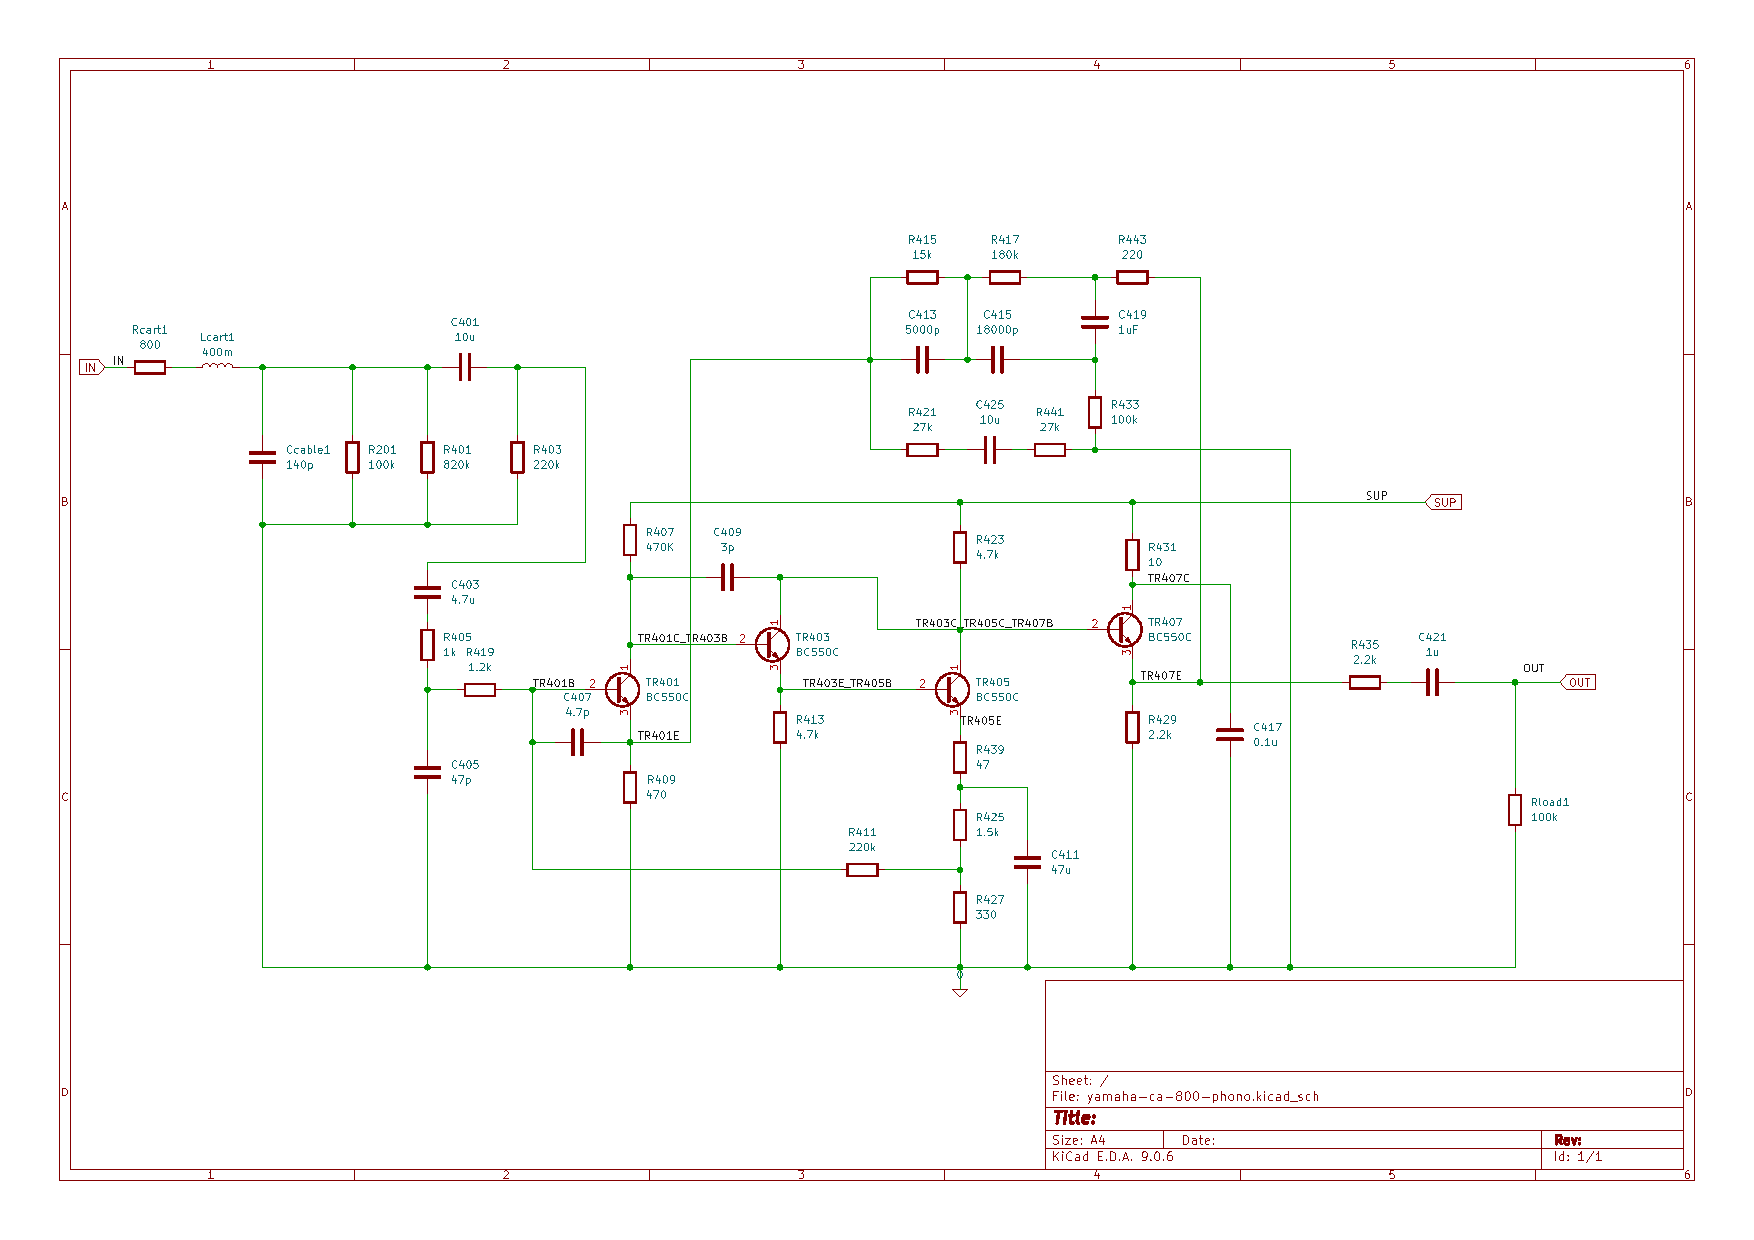
\includegraphics[width=\linewidth]{figures/yamaha-ca-800-phono.pdf}
	\caption{Schematics for simulation}
	\label{fig:simu}
\end{figure}

\begin{figure}[H]
	\centering
	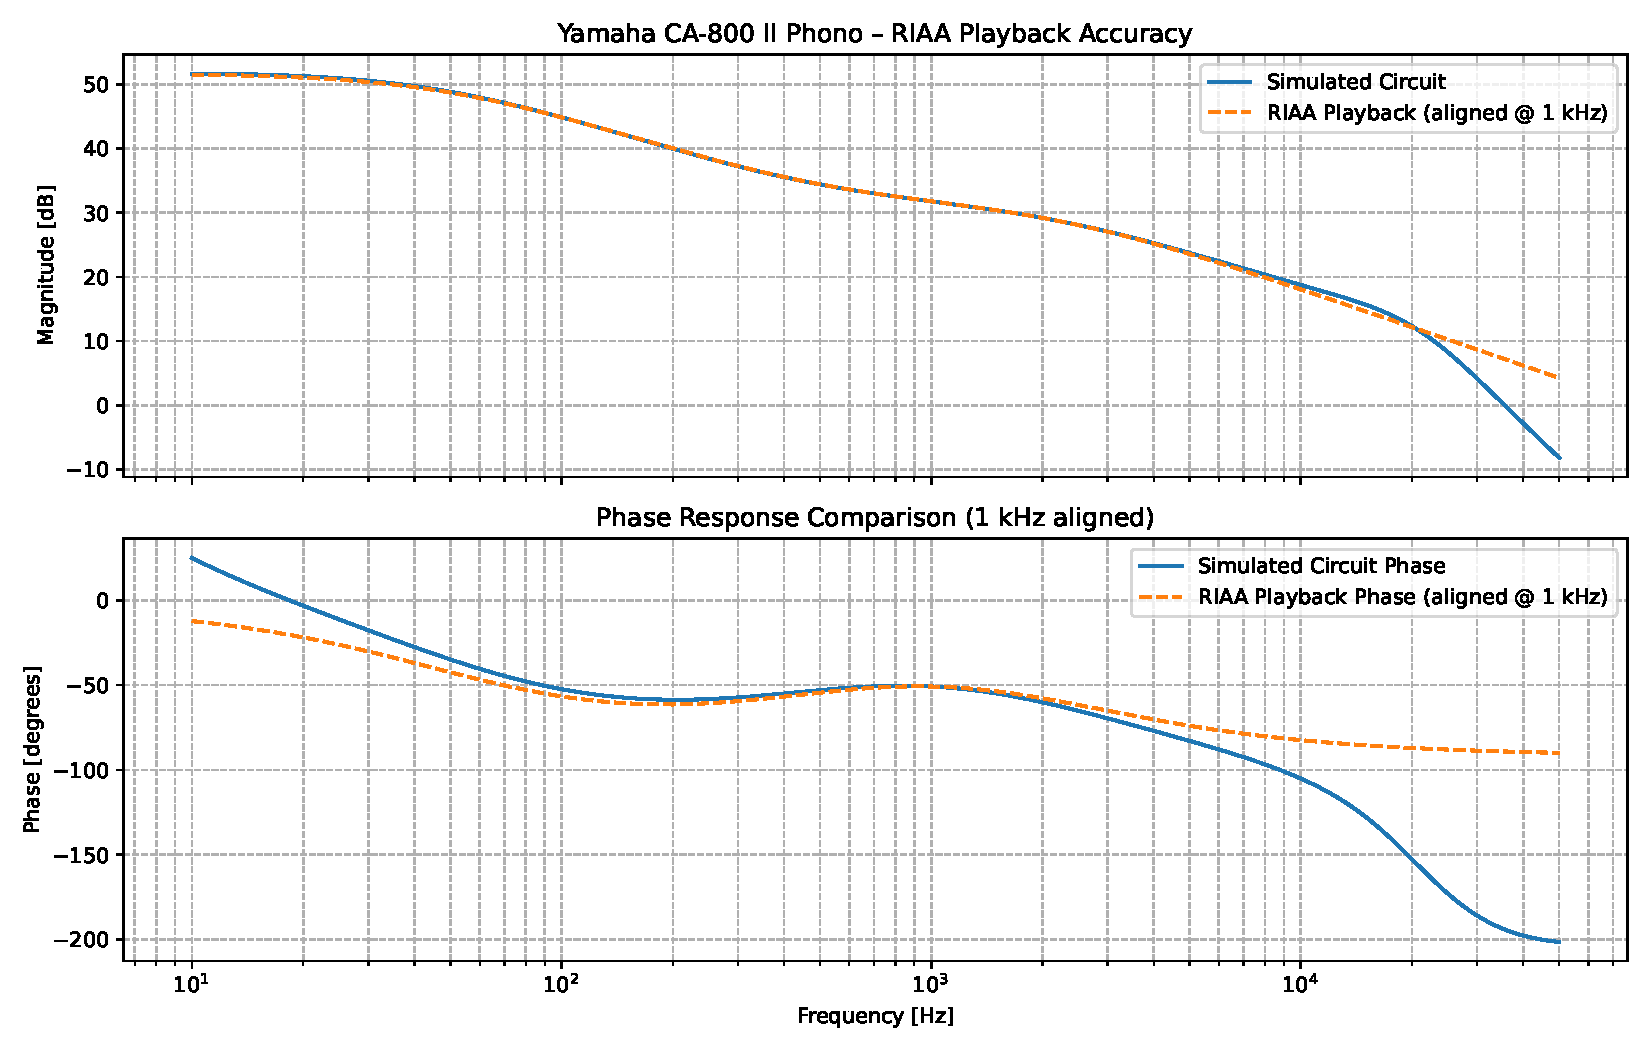
\includegraphics[width=\linewidth]{figures/riaa.pdf}
	\caption{Simulation of the phono preamplifier with a 400\,mH cartridge using the modified component values.}
	\label{fig:simu}
\end{figure}

\begin{table}[H]
	\centering
	\caption{Function Board Repair Log}
	\label{tab:repair_log_function_board}
	\begin{tabular}{|l|l|l|}
		\hline
		\textbf{Ref.} & \textbf{Original} & \textbf{Replacement} \\
		\hline
		TR401, TR402 & 2SC1345 & KSC1845F (HFE $\approx$ 500) \\
		TR403, TR404 & 2SC1345 & KSC1845F (HFE $\approx$ 500) \\
		TR405, TR406 & 2SC1345 & KSC1845F (HFE $\approx$ 500) \\
		TR407, TR408 & 2SC1166 & TTC004B (HFE $\approx$ 180) \\
		\hline
		C405, C406 & 100\,pF & 3\,pF \\
		C407, C408 & 3\,pF & 47\,pF \\
		C409, C410 & 3\,pF & 47\,pF \\
		C411, C412 &   & 47\,$\mu$F / 25\,V (Kemet A750EK476M1EAAE040) \\
		C401, C402 &   & 10\,$\mu$F / 25\,V (Kemet A758BG106M1EAAE070) \\
		C403, C404 &   & 10\,$\mu$F / 25\,V (Kemet A758BG106M1EAAE070) \\
		C413, C414 & 5000\,pF & 3300\,pF \\
		C415, C416 & 18\,nF & 12\,nF \\
		C417, C418 & 4.7\,$\mu$F & 1\,$\mu$F / 50\,V (Kemet ESC105M050AC3AA) \\
		C241 &   & 220\,$\mu$F / 50\,V (Panasonic EEU-FR1H221B) \\
		\hline
		R413, R414 & 15\,k$\Omega$ & 18\,k$\Omega$ \\
		R415, R416 & 180\,k$\Omega$ & 330\,k$\Omega$ \\
		\hline
	\end{tabular}
\end{table}

\begin{table}[H]
	\centering
	\caption{Function board transistor voltages. Measured values are shown first; values in parentheses correspond to the ngspice simulation and Yamaha service manual, respectively.}
	\label{tab:function_board_voltages}
	\begin{tabular}{|l|l|l|l|}
    \hline
 \textbf{Ref.} & \textbf{B} & \textbf{E} & \textbf{C} \\
    \hline
    TR401 & 0.66V (0.63V) & 0.08V (130mV; 0.2V)  & 5.09V (5.17V; 9V) \\
    TR402 & 0.65V (0.63V) & 0.08V (130mV; 0.2V) & 5.08V (5.17V; 9V) \\
    TR403 & 5.07V (5.17V; 9V) & 4.52V (4.58V; 8V) & 26.7V (36.2V; 30.5V)  \\
    TR404 & 5.04V (5.17V; 9V) & 4.5V (4.58V; 8V)  & 27.07V (36.2V; 30.5V) \\
    TR405 & 4.5V (4.58V; 8V) & 3.89V (3.97V; 7.5) & 26.7V (36.2V; 30.5V)  \\
    TR406 & 4.49V (4.58V; 8V) & 3.88V (3.97V; 7.5V) & 27.08V (36.2V; 30.5V) \\
    TR407 & 27.2V (36.2V; 30.5V)  & 26.7V (35.5V; 30V) & 49.5V (50.8V; 51V) \\
    TR408 & 27.6V (36.2V; 30.5V) & 27.08V (35.5V; 30V) & 49.5V (50.8V; 51V) \\
    \hline
	\end{tabular}
\end{table}

The measured transistor voltages show reasonable agreement with both the ngspice simulation and the Yamaha service manual values. Remaining discrepancies are expected because the simulation uses simplified transistor models and modern replacement devices rather than the original Yamaha transistors. Additional variation is introduced by component tolerances, supply-voltage differences, and production variations between amplifier revisions.

Although some collector voltages differ noticeably from the service manual and simulation results, all transistor stages remain correctly biased and operate in their forward-active region under normal phono operating conditions. No evidence of transistor saturation or cutoff was observed during simulation or measurement, indicating that the modified phono stage maintains proper linear operation across the intended signal range.

\begin{table}[H]
\centering
\caption{Estimated transistor thermal behaviour from measured DC operating points}
\label{tab:function_board_transistor_thermal}
\begin{tabular}{|l|l|r|r|r|r|}
\hline
\textbf{Ref.} & \textbf{Type} & \textbf{$P_D$} & \textbf{$R_{\theta JA}$} & \textbf{$\Delta T_J$} & \textbf{$T_J$ at 40\,°C} \\
\hline
TR401, TR402 & KSC1845F & 0.85\,mW & 250\,°C/W & 0.2\,°C & 40.2\,°C \\
TR403, TR404 & KSC1845F & 22\,mW & 250\,°C/W & 5.5\,°C & 45.5\,°C \\
TR405, TR406 & KSC1845F & 88\,mW & 250\,°C/W & 22\,°C & 62\,°C \\
TR407, TR408 & TTC004B & 277\,mW & 100\,°C/W & 28\,°C & 68\,°C \\
\hline
\end{tabular}
\end{table}

\section{Tone control board}

The capacitance and ESR of all electrolytic capacitors were measured, and any capacitor was replaced if a new component provided significantly lower ESR.

\begin{table}[H]
	\centering
	\caption{Tone Control Board Repair Log}
	\label{tab:repair_log_tone_control_board}
	\begin{tabular}{|l|l|l|}
		\hline
		\textbf{Ref.} & \textbf{Original} & \textbf{Replacement} \\
		\hline
		TR301, TR302 & 2SC1345D & KSC1845F (HFE $\approx$ 400) \\
        TR303, TR304 & 2SA763WL4 & KSA992F (HFE $\approx$ 400) \\
		TR305, TR306 & 2SC1345D & KSC1845F (HFE $\approx$ 400) \\
        TR307, TR308 & 2SA763WL4 & KSA992F (HFE $\approx$ 400) \\
        TR309, TR310 & 2SA763WL4 & KSA992F (HFE $\approx$ 400) \\
		TR311, TR312 & 2SC1345D & KSC1845F (HFE $\approx$ 400) \\
		\hline
		C347 &  &   220\,$\mu$F / 50\,V (Panasonic EEU-FR1H221B) \\
		C325, C325& & 10\,$\mu$F / 25\,V (Kemet A758BG106M1EAAE070) \\
		\hline
	\end{tabular}
\end{table}

\section{Filter Board}

The capacitance and ESR of all electrolytic capacitors were measured, and any capacitor was replaced if a new component provided significantly lower ESR.

\begin{table}[H]
	\centering
	\caption{Filter Board Repair Log}
	\label{tab:repair_log_filter_board}
	\begin{tabular}{|l|l|l|}
		\hline
		\textbf{Ref.} & \textbf{Original} & \textbf{Replacement} \\
		\hline
		TR501, TR502 & 2SC1345D & KSC1845F (HFE $\approx$ 400) \\
		TR505, TR506 & 2SC1345D & KSC1845F (HFE $\approx$ 400) \\
		\hline
		C526 &  &   220\,$\mu$F / 50\,V (Panasonic EEU-FR1H221B) \\
		C325, C325& & 10\,$\mu$F / 25\,V (Kemet A758BG106M1EAAE070) \\
		\hline
	\end{tabular}
\end{table}

\section{Operation Switch Circuit Board}

The two broken microswitches were replaced with Omron OM V-15-1A5 switches.

\section{Main Board}

The Yamaha CA-800 II uses separate main amplifier boards for the left and right channels. On both boards, the alignment procedure was performed according to the instructions given in the official service manual. After adjustment, the transistor operating voltages were measured and compared against the documented reference values.

In the following tables, the voltages shown in parentheses correspond to the expected values specified in the service manual. For transistors with two measurement rows, the upper row corresponds to operation in Class AB mode, while the lower row corresponds to operation in Class A mode.

Only a small number of components required replacement on the main amplifier boards. The replaced capacitors are located in positions related to signal coupling, feedback, and amplifier stability. After servicing, both amplifier channels showed stable operation and good agreement with the expected operating points.


\subsection{Left Channel}

The left main amplifier board was serviced and aligned according to the factory adjustment procedure. Capacitors C601, C605, and C611 were replaced with modern equivalents of suitable electrical specification.

The measured transistor voltages show good agreement with the reference values from the service manual. Minor deviations are considered acceptable and are consistent with normal component tolerances, semiconductor variation, and differences in measurement conditions.

\begin{table}[H]
	\centering
	\caption{Main Amp Left Repair Log}
	\label{tab:repair_log_main_left}
	\begin{tabular}{|l|l|l|}
		\hline
		\textbf{Ref.} & \textbf{Original} & \textbf{Replacement} \\
		\hline
		C601 &  &   2.2\,$\mu$F / 50\,V (Panasonic ECEA1HN470U) \\
        C605 &  &   47\,$\mu$F / 50\,V (Panasonic ECEA1HN2R2U)\\ 
		C611 &  &   0.47\,$\mu$F / 63\,VAC 100\,VDC (Kemet R82EC3470AA70J) \\
        
		\hline
	\end{tabular}
\end{table}

\begin{table}[H]
	\centering
	\caption{Main Amp Left Voltages}
	\label{tab:main_amp_left_voltages}
	\begin{tabular}{|l|l|l|l|}
    \hline
 \textbf{Ref.} & \textbf{B} & \textbf{E} & \textbf{C} \\
    \hline
    TR601 (pnp) & 12mV (20mV) & 571mV (0.5V) & -51.42V (-53V)  \\
    \hline
    TR602 (npn) & -51.45V (-53.5V) & -52V (-54V) & -51.33V (-53V)  \\
    \hline
    TR603 (pnp) & 45.3V (47V) & 45.9V (47.5V) & 0.56V (0.5V) \\
    \hline
    TR604 (pnp) & 20mV (15mV) & 0.57V (0.5V) & -51.4V (-53V) \\
    \hline
    TR605 (npn) & -51.33V (-52V) & -51.8V (-53V) & -1.2V (-1.2V) \\
                & -51.2V (-52V)  & -51.8V (-53V) & -1.8V (-1.7V) \\
    \hline
    TR606 (pnp) & 1.1V (1V) & 1.76V (1.8V) & -1.25V (-1.2V) \\
                & 1.7V (1.7V) & 2.4V  & -1.77V (-1.7V) \\  
    \hline
    TR607 (npn) & -0.6V (-0.6V)  & -1.25V (-1.2V) & 1.16V (1V) \\
               & -1.13V (-1V)  & -1.73V (-1.7V) & 1.69V (1.7V) \\
    \hline
    TR608 (npn) & 10mV (100mV) & 3mV (0V)  & 1.55V (1.5V)   \\
                & 220mV (300mV)  & 3mV (0V) & 2.2V (2V)  \\
    \hline
    TR609 (pnp) & -140mV (-200mV) & 3mV  & -1V (-1V)  \\
                & -310mV  & 3mV  & -1.46V (-1.5V) \\
    \hline
    TR610 (npn) & 1.82V (1.7V) & 1.25V  & 43.24V (43V)  \\
                & 2.41V (2.4V) & 1.79V    & 17.8V   \\
    \hline
    TR611 (pnp) & -1.26V (-1.2V) & -0.66V (-0.6V) & -43.37V (-43V)  \\
                & -1.78V (-1.74V) & -1.13V (-1V) & -17.6V (-17.0V) \\
    \hline
    TR612 (npn) & 0.63V (0.6V) & 21mV (23mV) & 42.22V \\
                & 1.12V (1V) & 0.4V (0.41V) & 17.8V \\
    \hline
    TR613 (pnp) & -0.63V (-0.6V) & -20mV (-30mV)  & -42.52V   \\
                & -1.12V (-1V) & -0.41V (-0.44V)  & -17.7V  \\
    \hline
	\end{tabular}
\end{table}

\subsection{Right Channel}

The right main amplifier board was serviced and aligned according to the factory adjustment procedure. Capacitors C601, C605, and C611 were replaced with modern equivalents of suitable electrical specification.

The measured transistor voltages show good agreement with the reference values from the service manual. Minor deviations are considered acceptable and are consistent with normal component tolerances, semiconductor variation, and differences in measurement conditions.

\begin{table}[H]
	\centering
	\caption{Main Amp Right Repair Log}
	\label{tab:repair_log_main_right}
	\begin{tabular}{|l|l|l|}
		\hline
		\textbf{Ref.} & \textbf{Original} & \textbf{Replacement} \\
		\hline
		C601 &  &   2.2\,$\mu$F / 50\,V (Panasonic ECEA1HN470U) \\
        C605 &  &   47\,$\mu$F / 50\,V (Panasonic ECEA1HN2R2U)\\ 
		C611 &  &   0.47\,$\mu$F / 63\,VAC 100\,VDC (Kemet R82EC3470AA70J) \\
        
		\hline
	\end{tabular}
\end{table}

\begin{table}[H]
	\centering
	\caption{Main Amp Right Voltages}
	\label{tab:main_amp_right_voltages}
	\begin{tabular}{|l|l|l|l|}
    \hline
 \textbf{Ref.} & \textbf{B} & \textbf{E} & \textbf{C} \\
    \hline
    TR601 (pnp) & 16mV (20mV)  & 570mV (0.5V)  & -51.42V  (-53V)  \\
    \hline
    TR602 (npn) & -51.45V (-53.5V)  & -52.16V (-54V)  & -51.4V (-53V) \\
    \hline
    TR603 (pnp) & 45.4V (47V) &  45.96V (47.5V) & 0.56V (0.5V)  \\
    \hline
    TR604 (pnp) & 16mV (20mV)  & 0.57 (0.5V) & -51.45V  (-53V) \\
    \hline
    TR605 (npn) & -51.4V (-52V) & -52.05V (-53V) & -1.22V (-1.2V)  \\
                & -51.4V (-52V) & -52.05V (-53V) & -1.8V (-1.7V)  \\
    \hline
    TR606 (pnp) & 1.1V (1V) & 1.78V (1.8V) & -1.25V (-1.2V) \\
                & 1.74V (1.7V) & 2.42V  & -1.77V (-1.7V) \\  
    \hline
    TR607 (npn) & -0.58V (-0.6V)  & -1.22V (-1.2V) & 1.1V (1V) \\
               & -1.16V (-1V)  & -1.8V (-1.7V) & 1.75V (1.7V) \\
    \hline
    TR608 (npn) & 10mV (100mV)  & 3mV (0V) & 1.55V (1.5V)  \\
                & 280mV (300mV)  & 3mV (0V)  & 2.2V (2V)  \\
    \hline
    TR609 (pnp) & -100mV (-200mV) & 3mV  & -1.02V (-1V)  \\
                & -310mV  & 3mV  & -1.55V (-1.5V) \\
    \hline
    TR610 (npn) & 1.77V (1.7V)  & 1.2V  & 43.24V (43V)  \\
                & 2.40V (2.4V) & 1.79V    & 16.2V   \\
    \hline
    TR611 (pnp) & -1.22V (-1.2V) & -0.61V (-0.6V)  & -43.37V (-43V) V  \\ 
                & -1.80V (-1.74V) & -1.13V (-1V)  & -16.2V (-17.0V) \\
    \hline
    TR612 (npn) & 0.63V (0.6V) & 21mV (24mV) & 42.22V \\
                & 1.12V (1V) & 0.4V (0.41V) & 16.2V \\
    \hline
    TR613 (pnp) & -0.63V (-0.6V) & -20mV (-40mV)  & -42.52V  \\
                & -1.12V (-1V) & -0.41V (-0.44V)  & -16.2V  \\
    \hline
	\end{tabular}
\end{table}

\section{Final Measurements}

\subsection{Phono Stage}

The phono stage was evaluated using an inverse RIAA network driven by a low-distortion signal generator. The generator output level was set to \(450\,\mathrm{mV}_{\mathrm{rms}}\), with the inverse RIAA converter connected to the Phono~1 input of the amplifier. An \(8\,\Omega\) non-inductive load resistor was connected to the amplifier output, and the volume control was adjusted to produce approximately \(25\,\mathrm{W}\) output power. The same input level and volume setting were maintained throughout all measurements.

Measurements were performed using Yet Another Audio Analyzer (YAAA) with a \(192\,\mathrm{kHz}\) sampling rate and \(65536\)-point FFT analysis. The measurements characterize the complete signal path through the phono equalizer, tone amplifier, and power amplifier sections following restoration.

Overall, the phono stage demonstrates very good post-restoration behavior. Low-frequency distortion remains exceptionally low, with THD values near \(0.02\%\) in both channels. Across the midband and upper audio range, THD generally remains between \(0.02\%\) and \(0.05\%\), while THD+N rises moderately due to the higher gain structure and broader noise contribution of the phono equalizer stage. Harmonic spectra are dominated by low-order components, and no signs of instability or oscillation were observed during testing.

\subsubsection{Left Channel}

The left channel exhibits very low distortion at low frequencies, with clean harmonic structure and a stable broadband noise floor.

\begin{figure}[H]
    \centering
    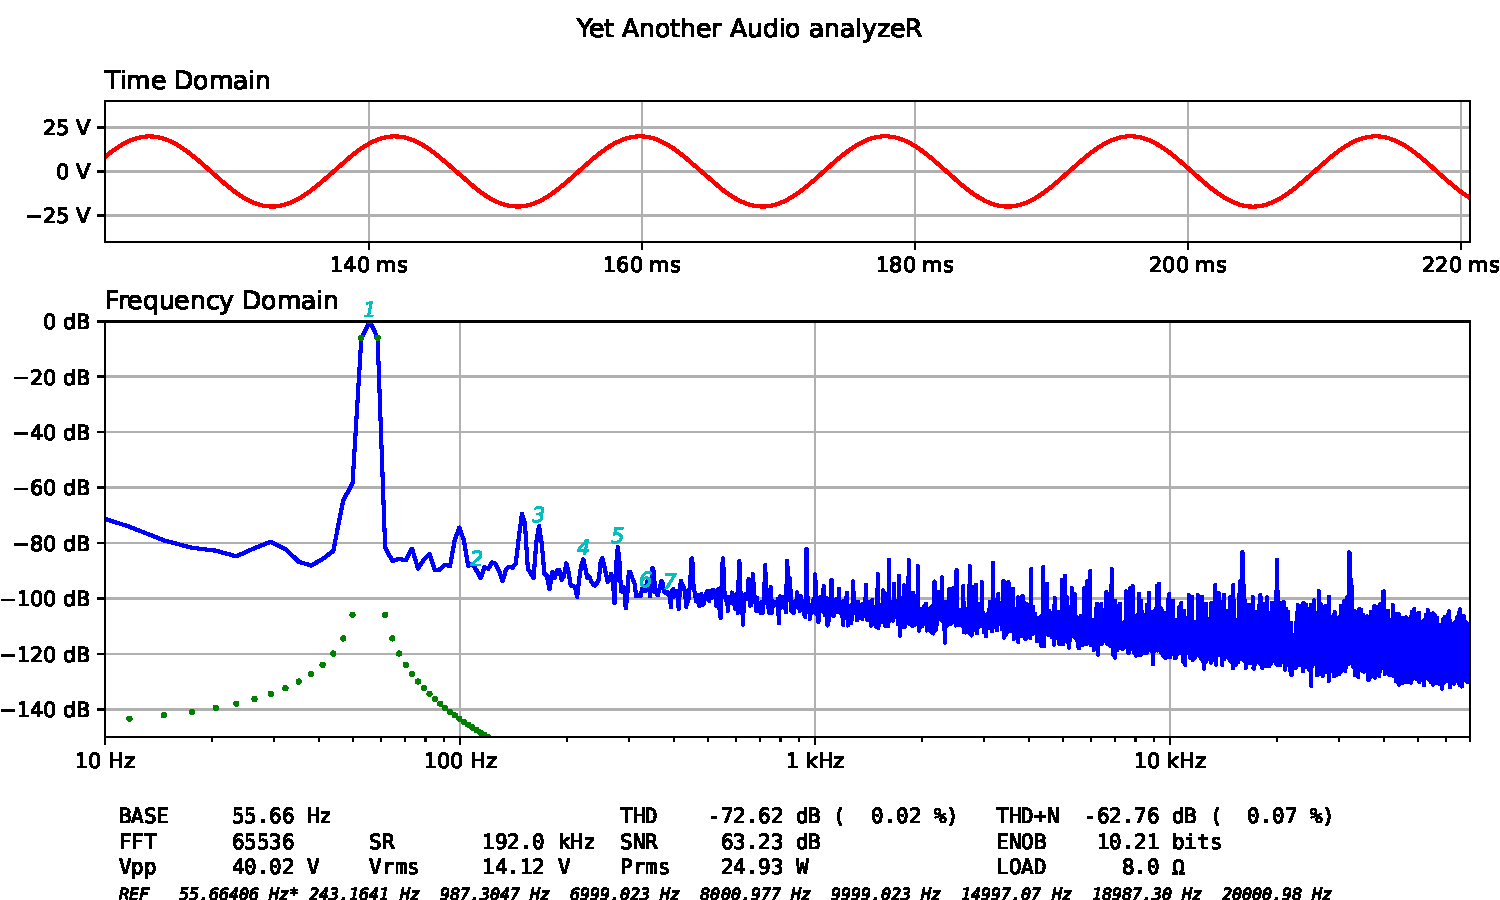
\includegraphics[width=0.95\textwidth]{measurements/yamaha_ca800ii_phono_left_56Hz_0Hz.pdf}
    \caption{Left channel phono-stage THD measurement at 55.66\,Hz.}
\end{figure}

\begin{figure}[H]
    \centering
    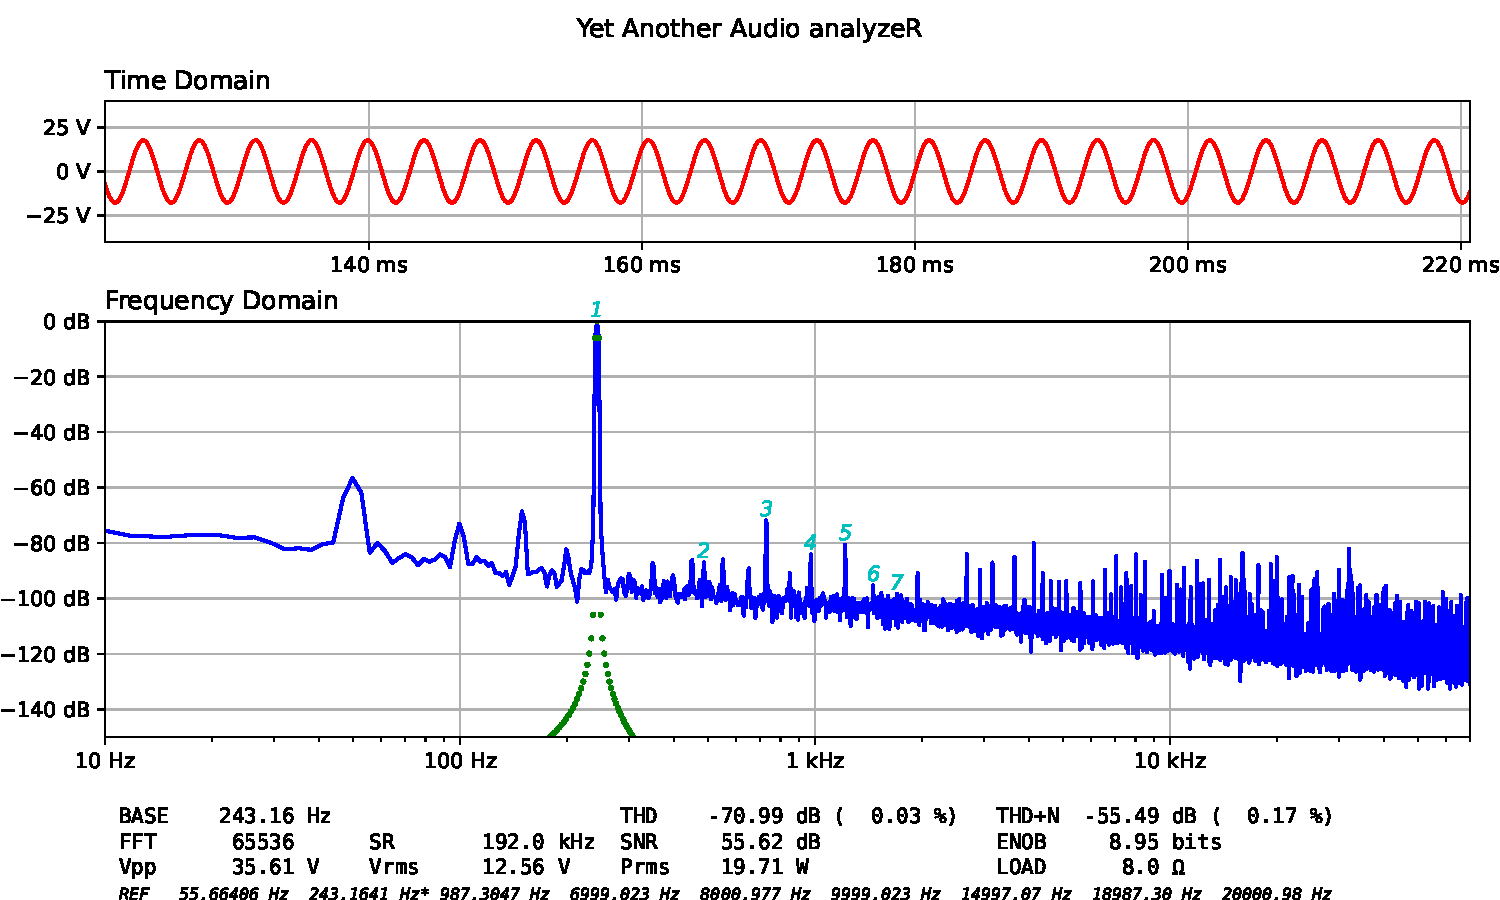
\includegraphics[width=0.95\textwidth]{measurements/yamaha_ca800ii_phono_left_243Hz_0Hz.pdf}
    \caption{Left channel phono-stage THD measurement at 243.16\,Hz.}
\end{figure}

Midband performance remains stable, with distortion products remaining well below audible thresholds.

\begin{figure}[H]
    \centering
    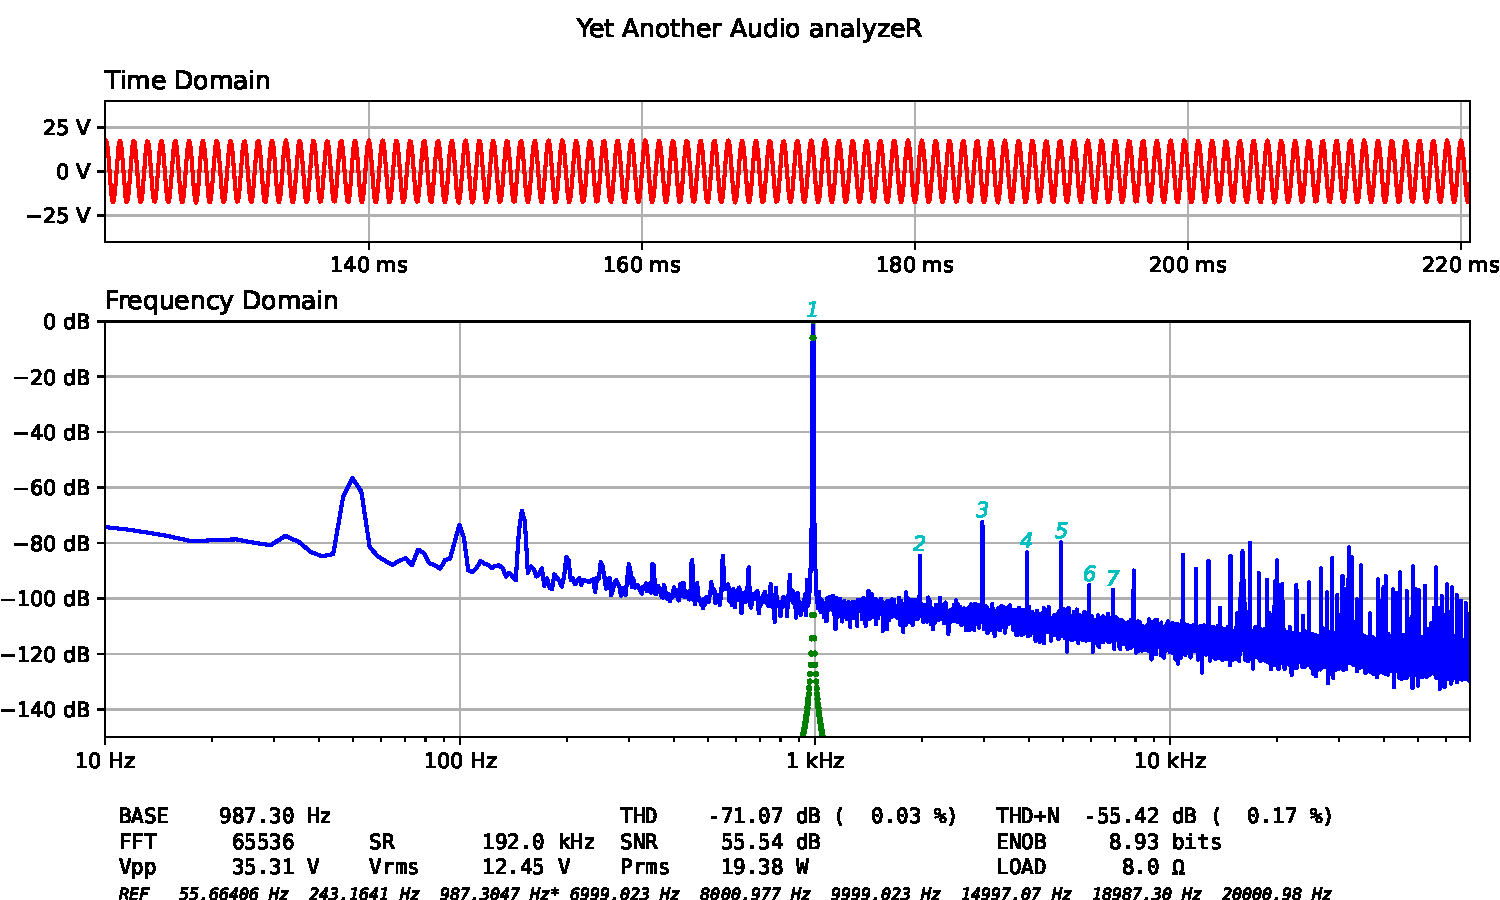
\includegraphics[width=0.95\textwidth]{measurements/yamaha_ca800ii_phono_left_987Hz_0Hz.pdf}
    \caption{Left channel phono-stage THD measurement at 987.30\,Hz.}
\end{figure}

At higher frequencies, the phono stage continues to maintain good linearity, although THD+N gradually increases as expected due to bandwidth limitations and increased wideband noise contribution.

\begin{figure}[H]
    \centering
    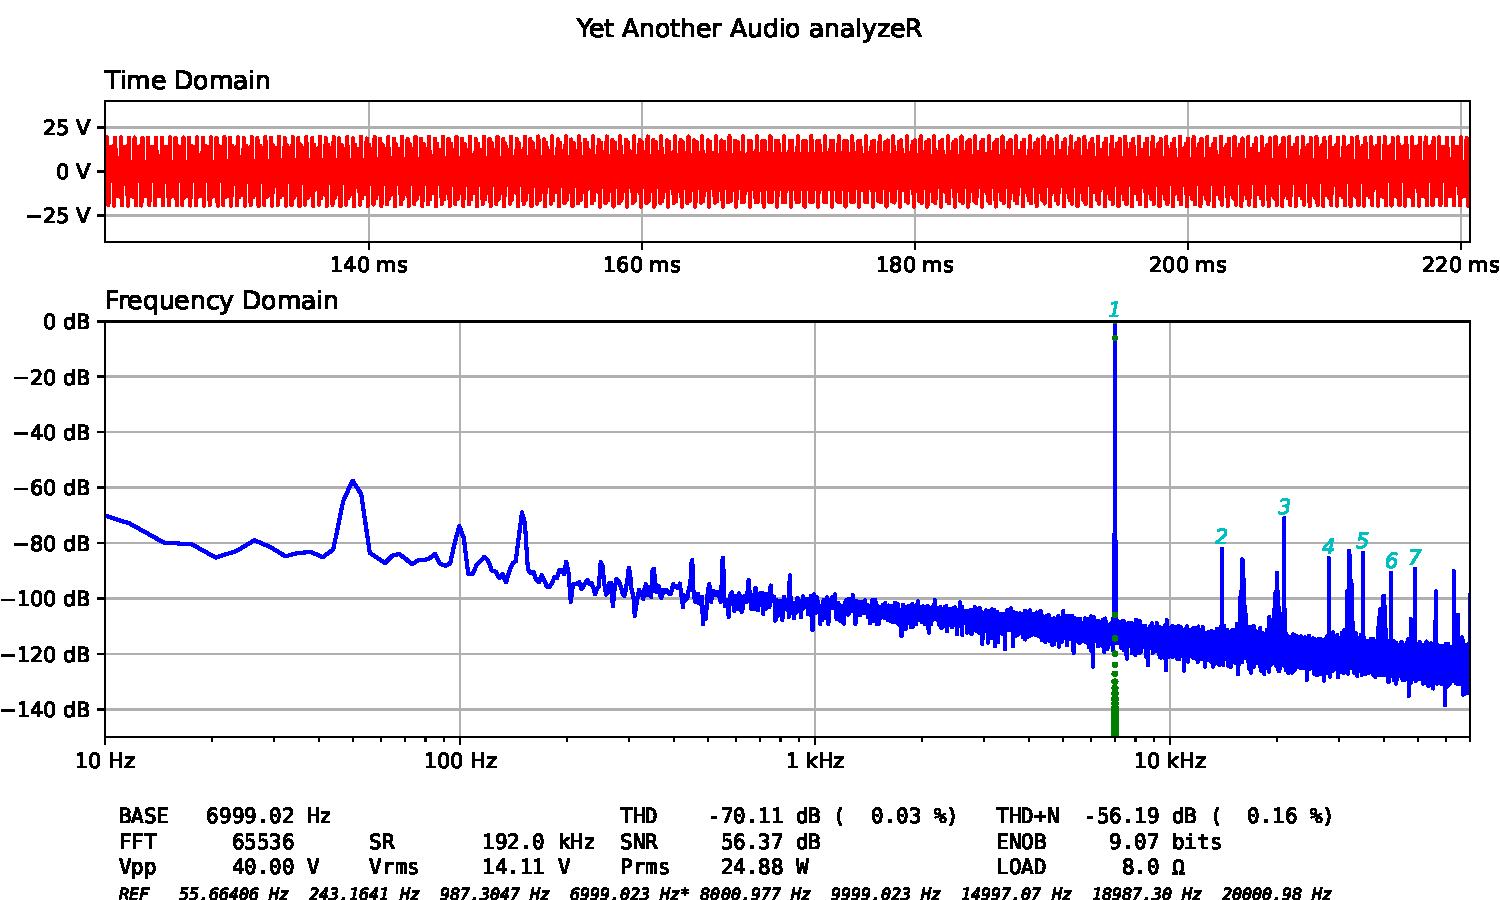
\includegraphics[width=0.95\textwidth]{measurements/yamaha_ca800ii_phono_left_6999Hz_0Hz.pdf}
    \caption{Left channel phono-stage THD measurement at 6.999\,kHz.}
\end{figure}

\begin{figure}[H]
    \centering
    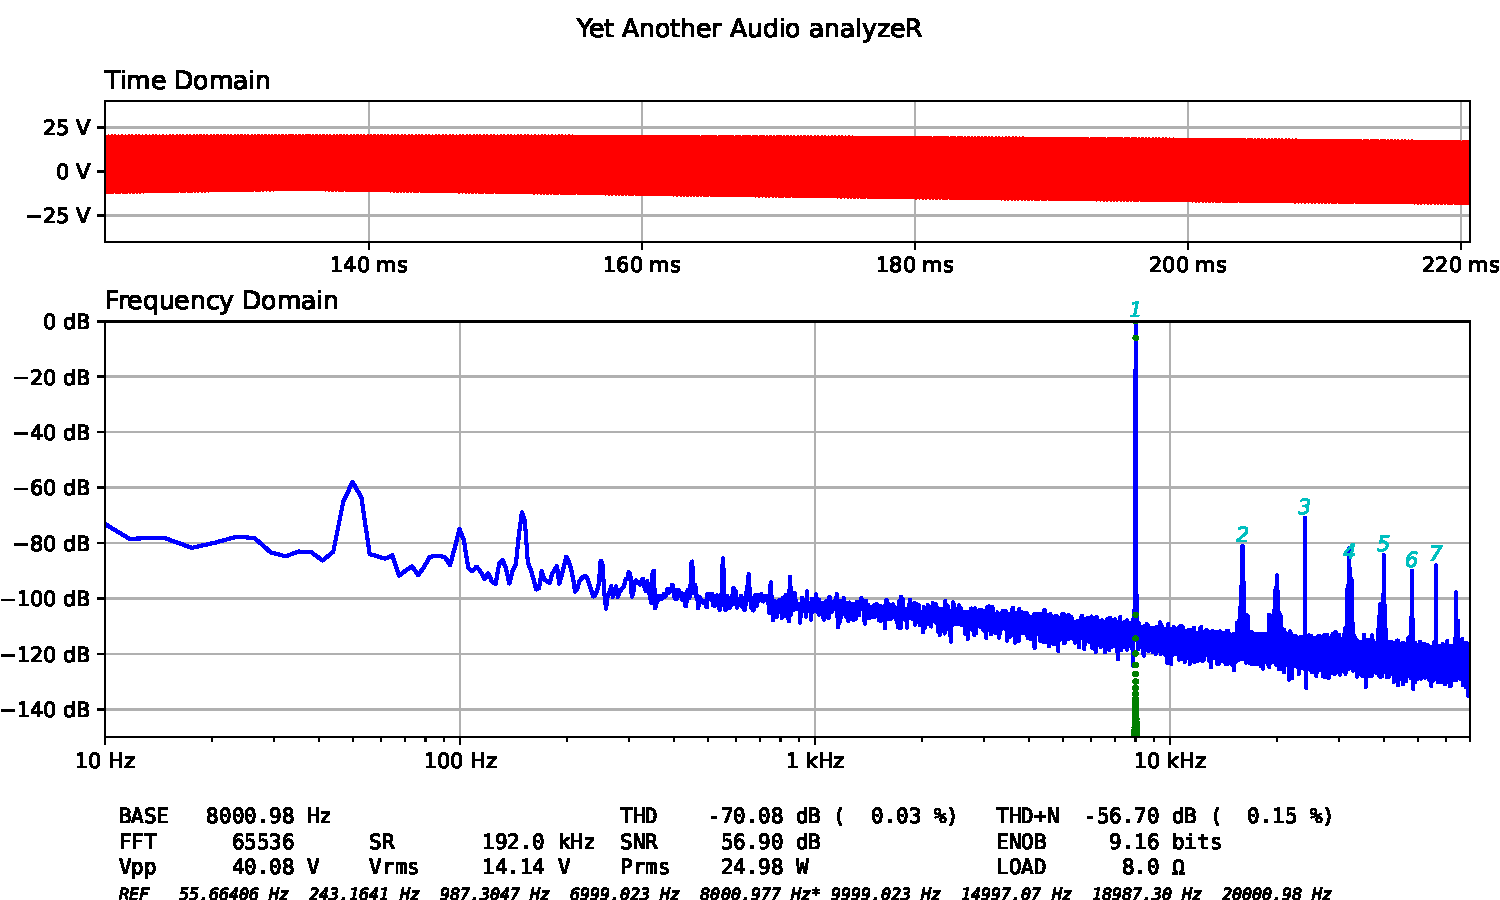
\includegraphics[width=0.95\textwidth]{measurements/yamaha_ca800ii_phono_left_8001Hz_0Hz.pdf}
    \caption{Left channel phono-stage THD measurement at 8.001\,kHz.}
\end{figure}

\begin{figure}[H]
    \centering
    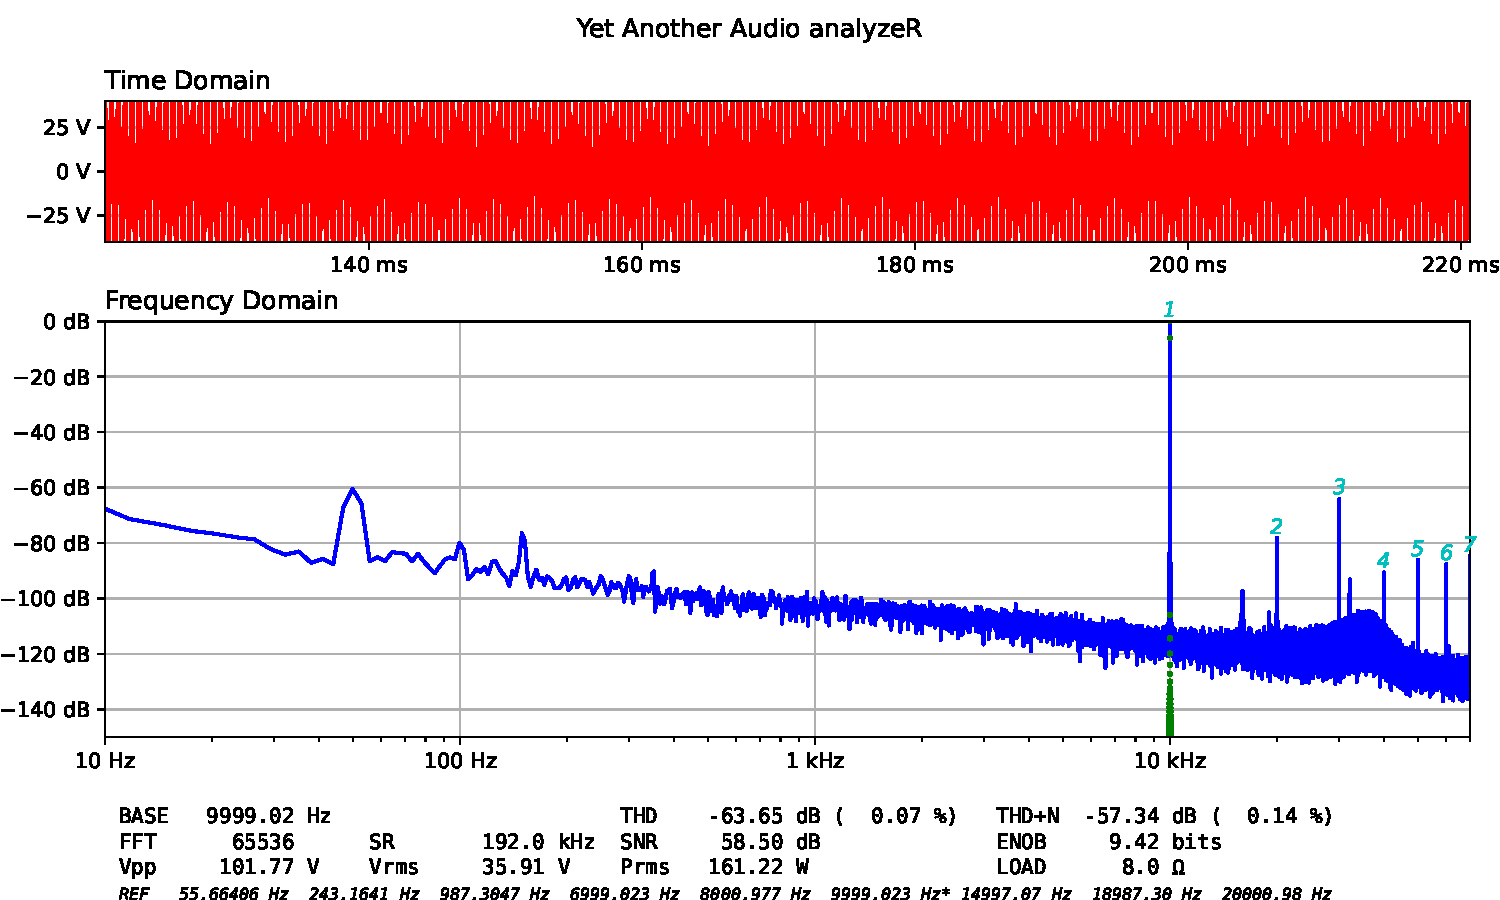
\includegraphics[width=0.95\textwidth]{measurements/yamaha_ca800ii_phono_left_9999Hz_0Hz.pdf}
    \caption{Left channel phono-stage THD measurement at 9.999\,kHz.}
\end{figure}

\begin{figure}[H]
    \centering
    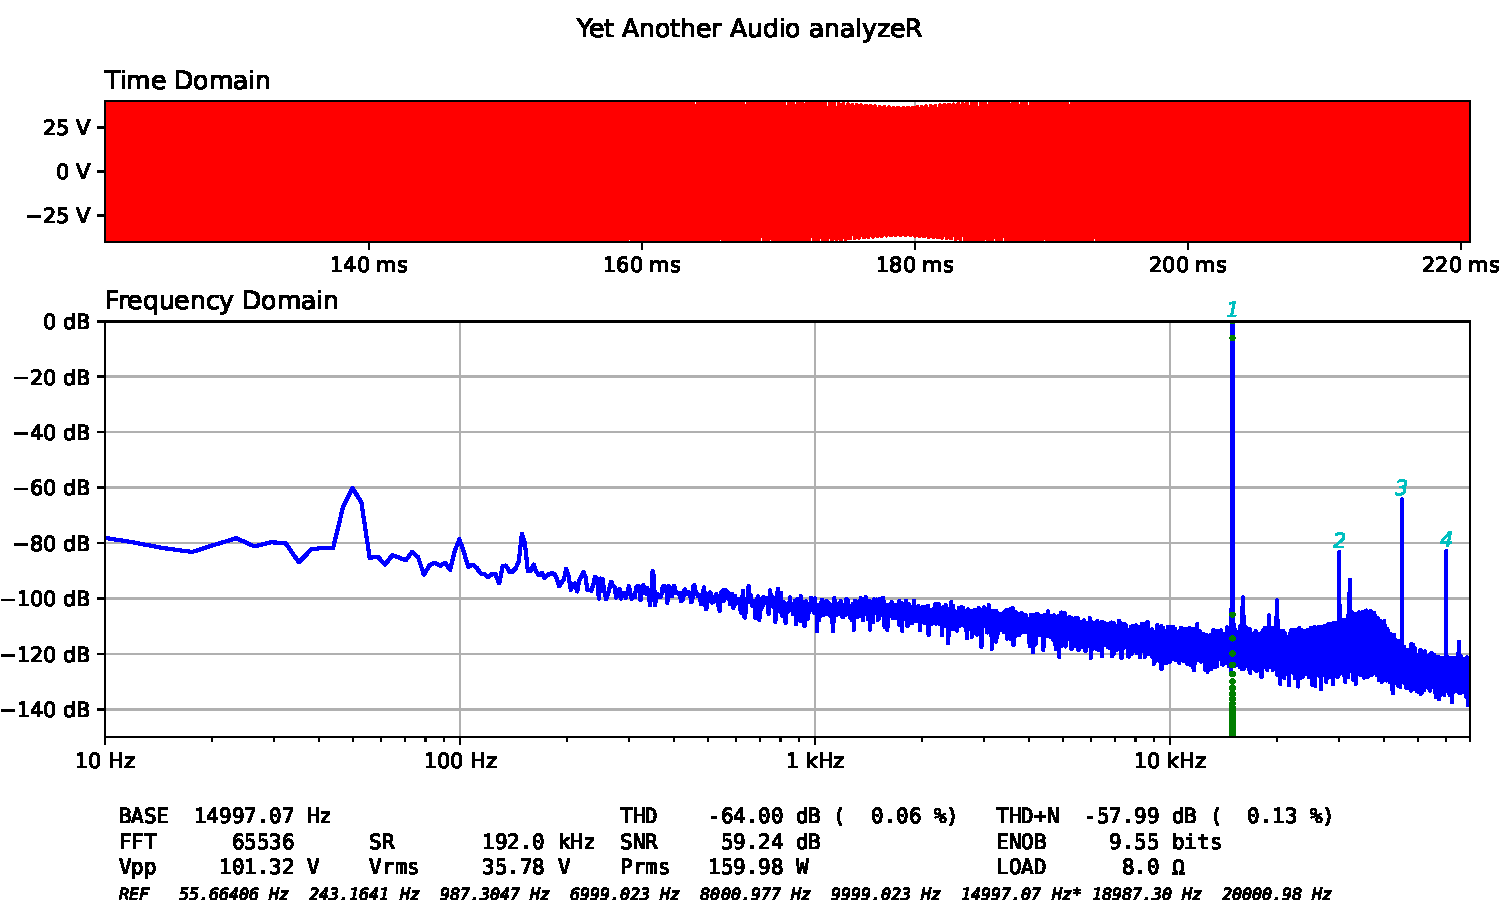
\includegraphics[width=0.95\textwidth]{measurements/yamaha_ca800ii_phono_left_14997Hz_0Hz.pdf}
    \caption{Left channel phono-stage THD measurement at 14.997\,kHz.}
\end{figure}

\begin{figure}[H]
    \centering
    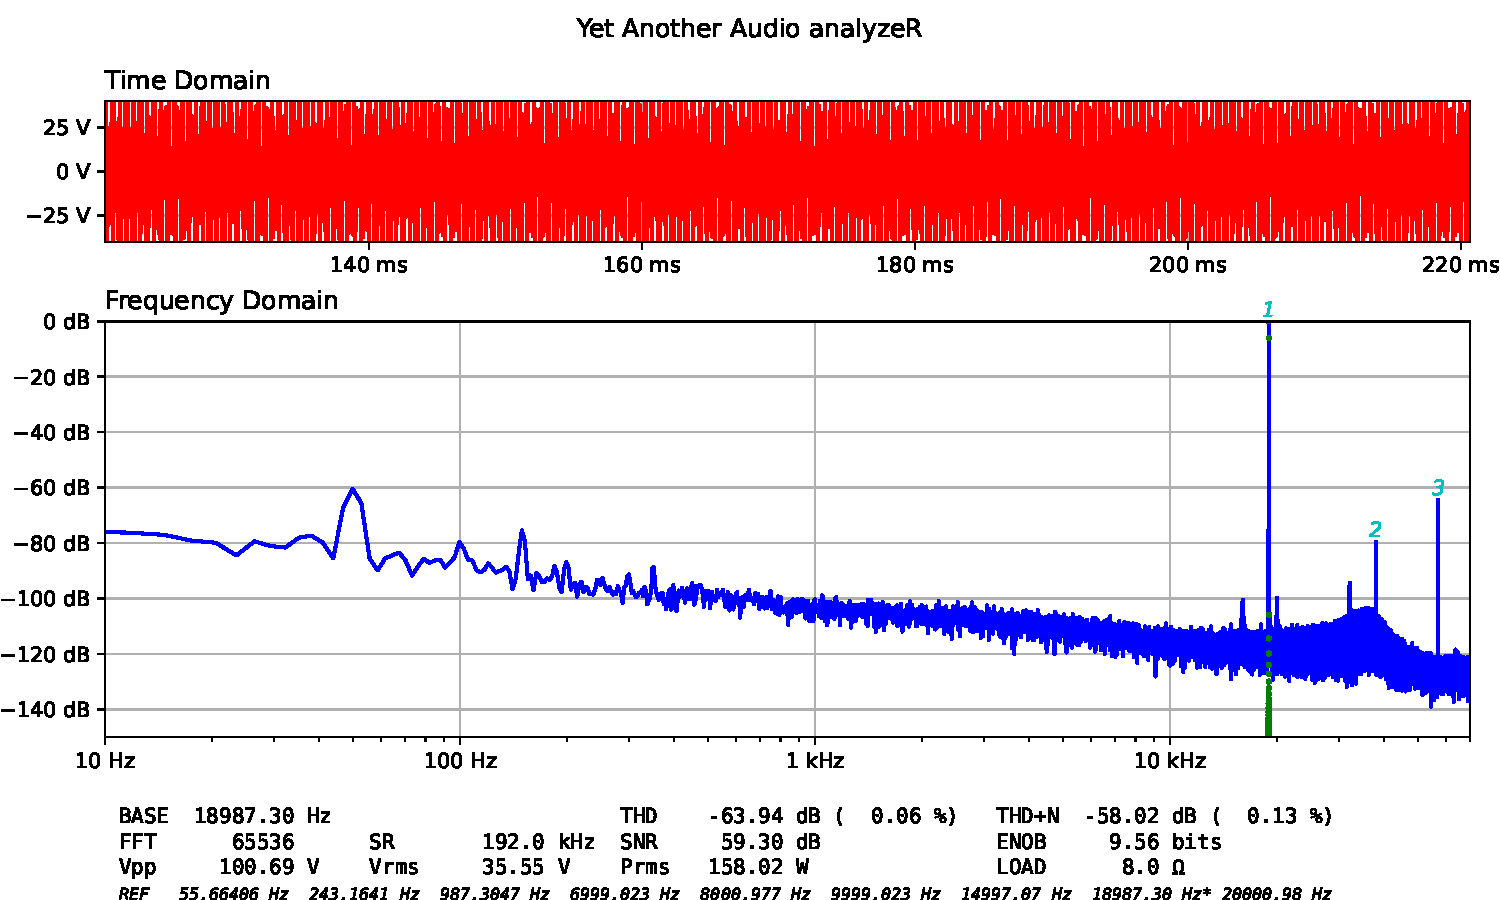
\includegraphics[width=0.95\textwidth]{measurements/yamaha_ca800ii_phono_left_18987Hz_0Hz.pdf}
    \caption{Left channel phono-stage THD measurement at 18.987\,kHz.}
\end{figure}

A CCIF twin-tone intermodulation test using 18.987\,kHz and 20.001\,kHz tones was also performed. The resulting spectrum shows extremely low CCIF products and very low SMPTE intermodulation distortion.

\begin{figure}[H]
    \centering
    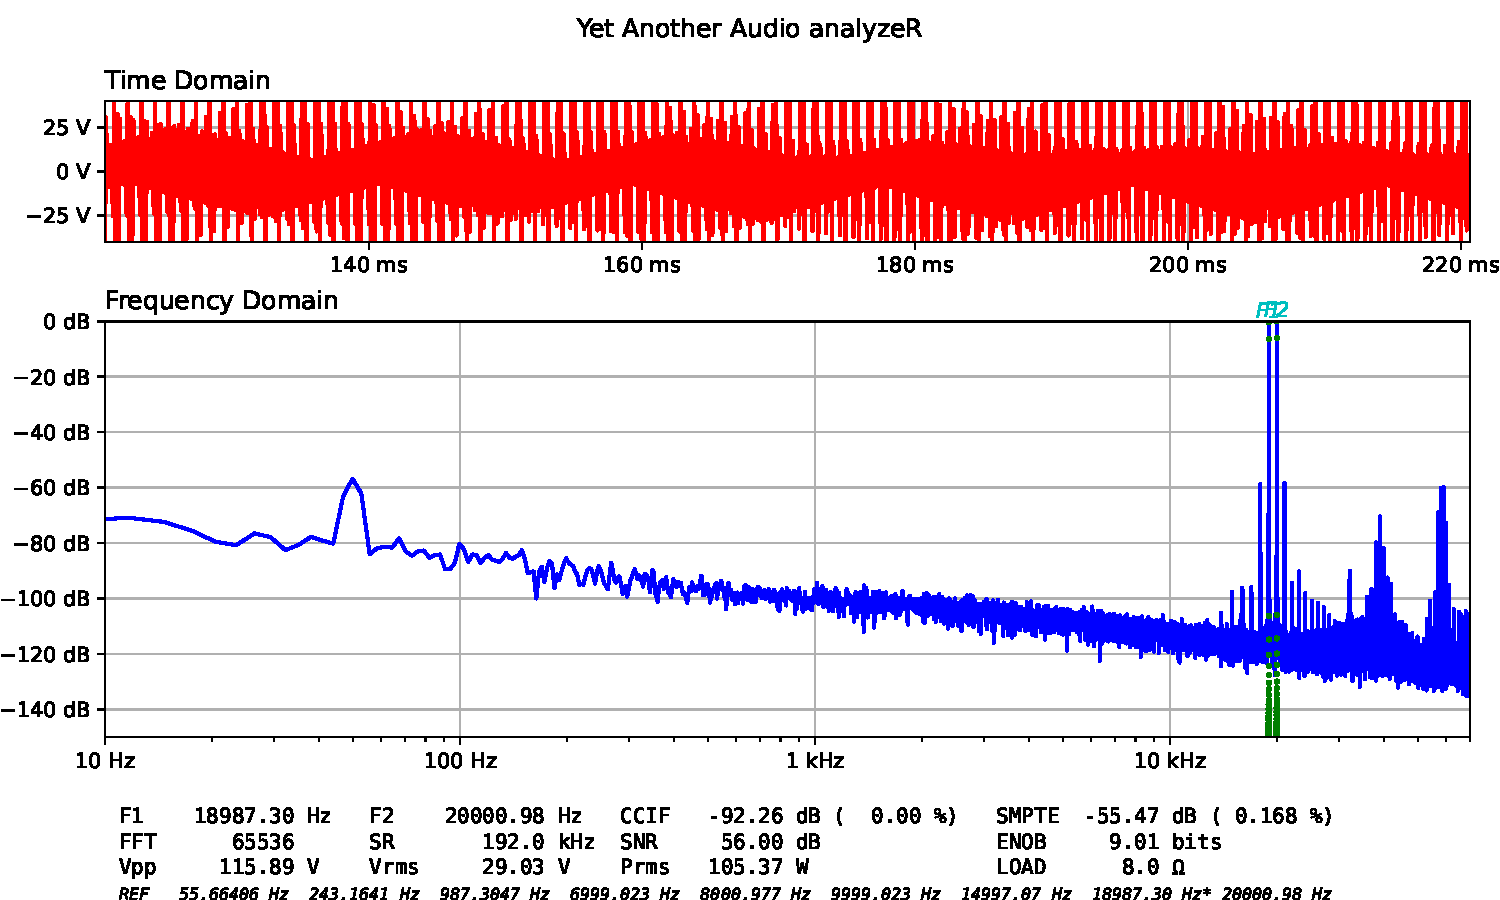
\includegraphics[width=0.95\textwidth]{measurements/yamaha_ca800ii_phono_left_18987Hz_20001Hz.pdf}
    \caption{Left channel phono-stage CCIF/SMPTE IMD measurement.}
\end{figure}

\subsubsection{Right Channel}

The right channel demonstrates similarly low distortion and closely matched spectral behavior throughout the measured frequency range.

\begin{figure}[H]
    \centering
    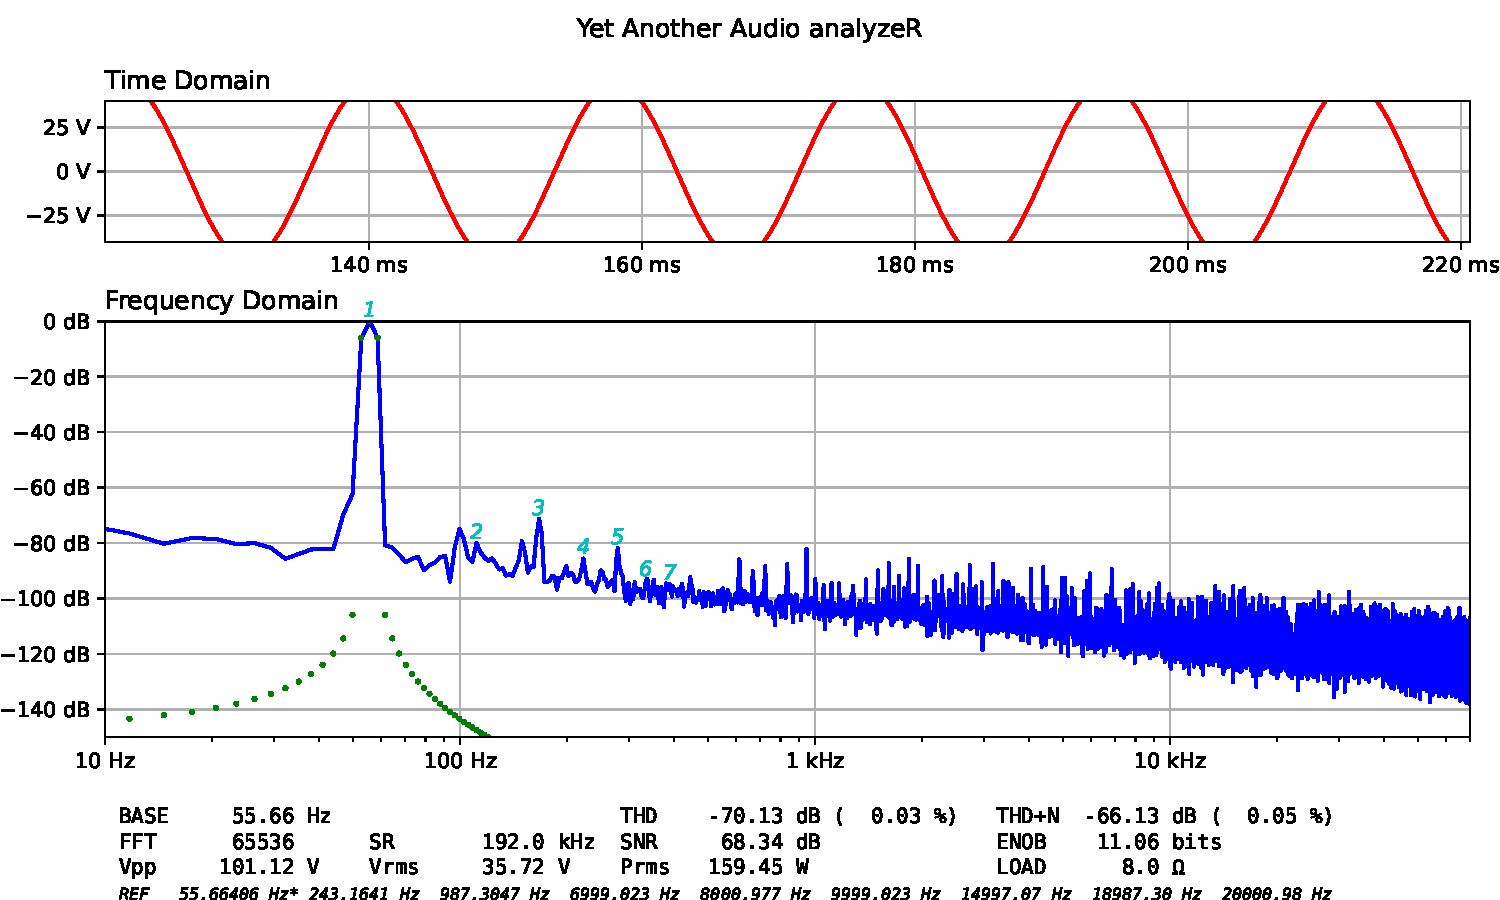
\includegraphics[width=0.95\textwidth]{measurements/yamaha_ca800ii_phono_right_56Hz_0Hz.pdf}
    \caption{Right channel phono-stage THD measurement at 55.66\,Hz.}
\end{figure}

\begin{figure}[H]
    \centering
    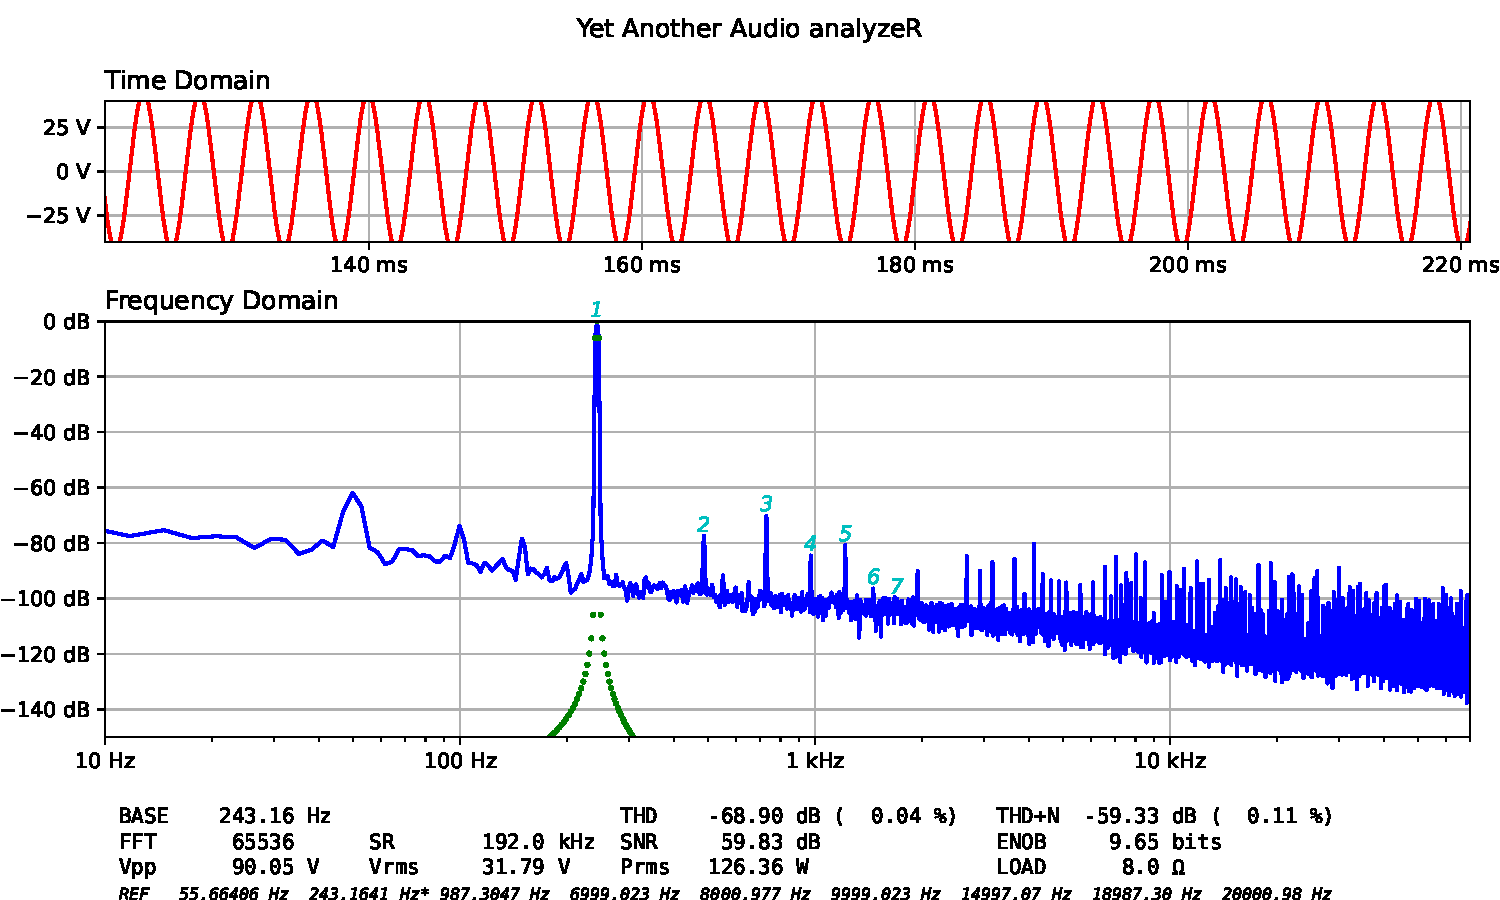
\includegraphics[width=0.95\textwidth]{measurements/yamaha_ca800ii_phono_right_243Hz_0Hz.pdf}
    \caption{Right channel phono-stage THD measurement at 243.16\,Hz.}
\end{figure}

\begin{figure}[H]
    \centering
    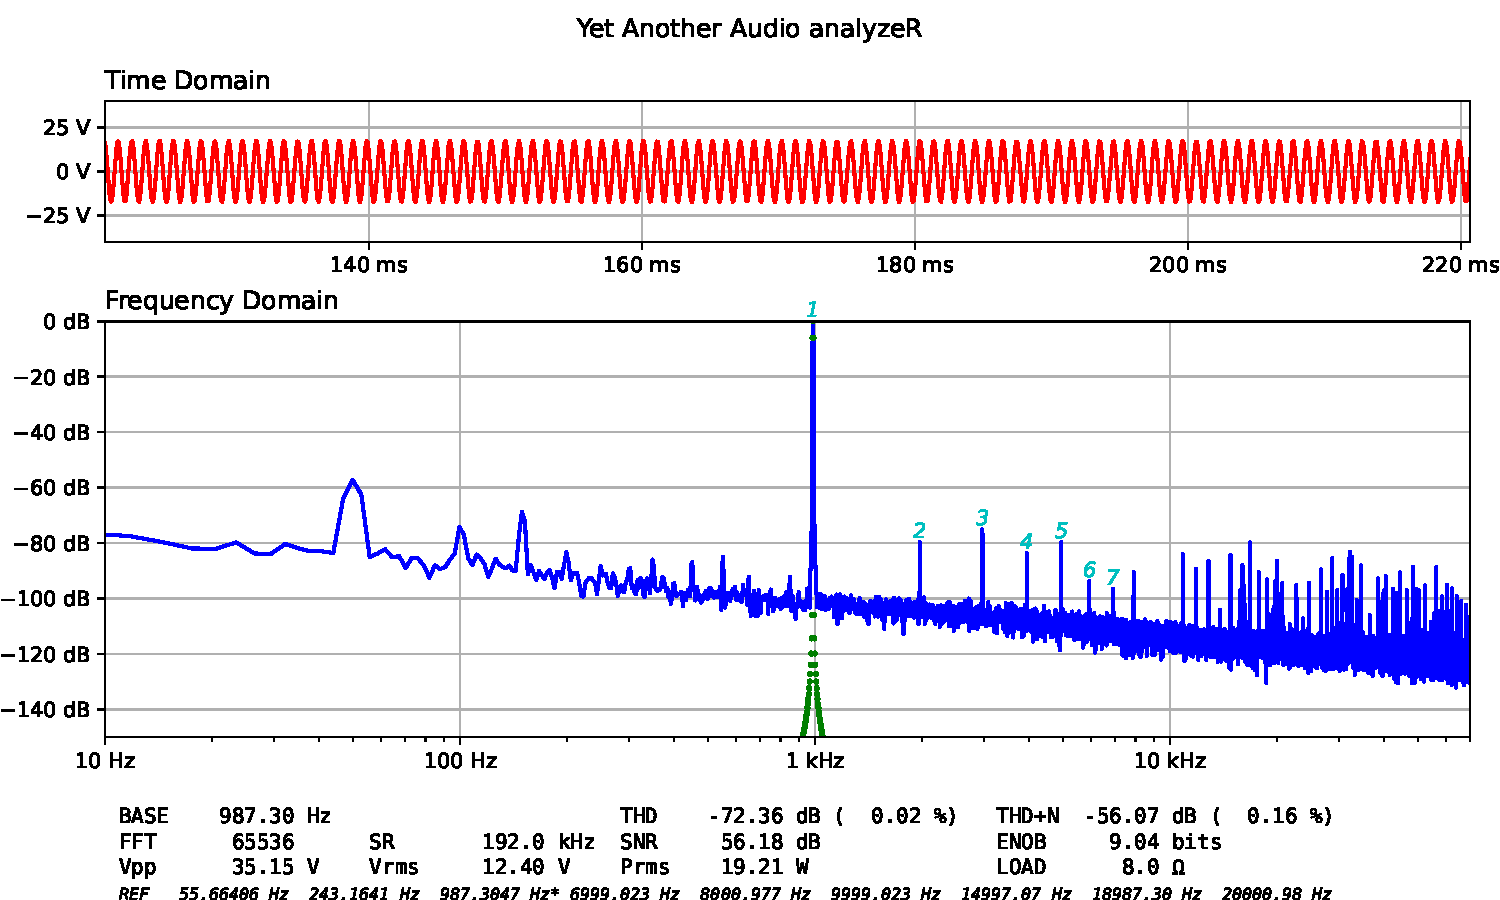
\includegraphics[width=0.95\textwidth]{measurements/yamaha_ca800ii_phono_right_987Hz_0Hz.pdf}
    \caption{Right channel phono-stage THD measurement at 987.30\,Hz.}
\end{figure}

At higher frequencies, the right channel maintains stable operation with only moderate increases in THD+N toward the upper edge of the audio band.

\begin{figure}[H]
    \centering
    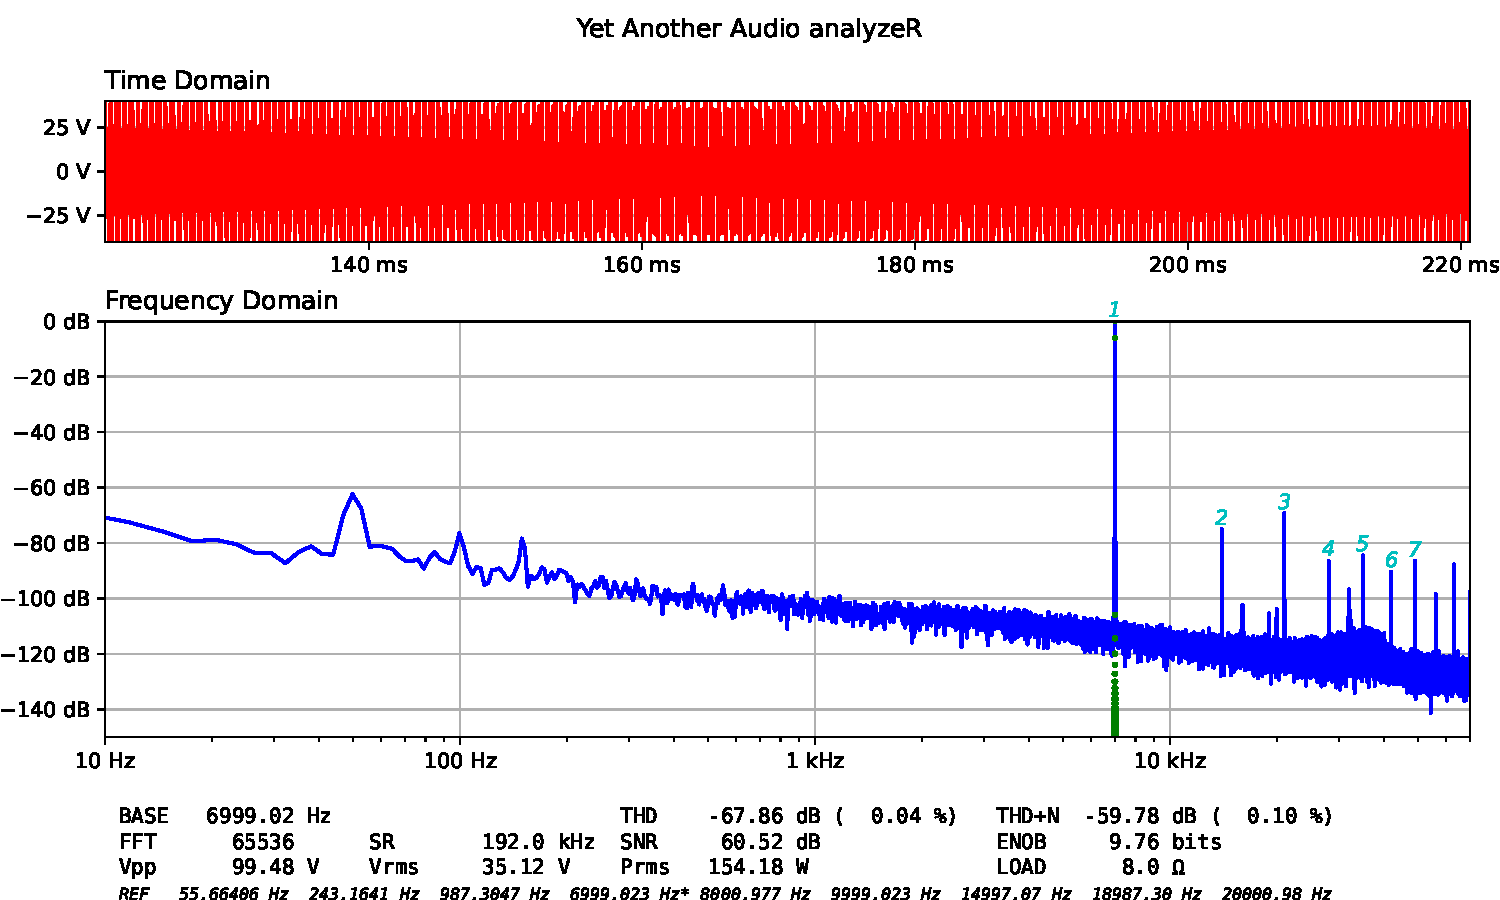
\includegraphics[width=0.95\textwidth]{measurements/yamaha_ca800ii_phono_right_6999Hz_0Hz.pdf}
    \caption{Right channel phono-stage THD measurement at 6.999\,kHz.}
\end{figure}

\begin{figure}[H]
    \centering
    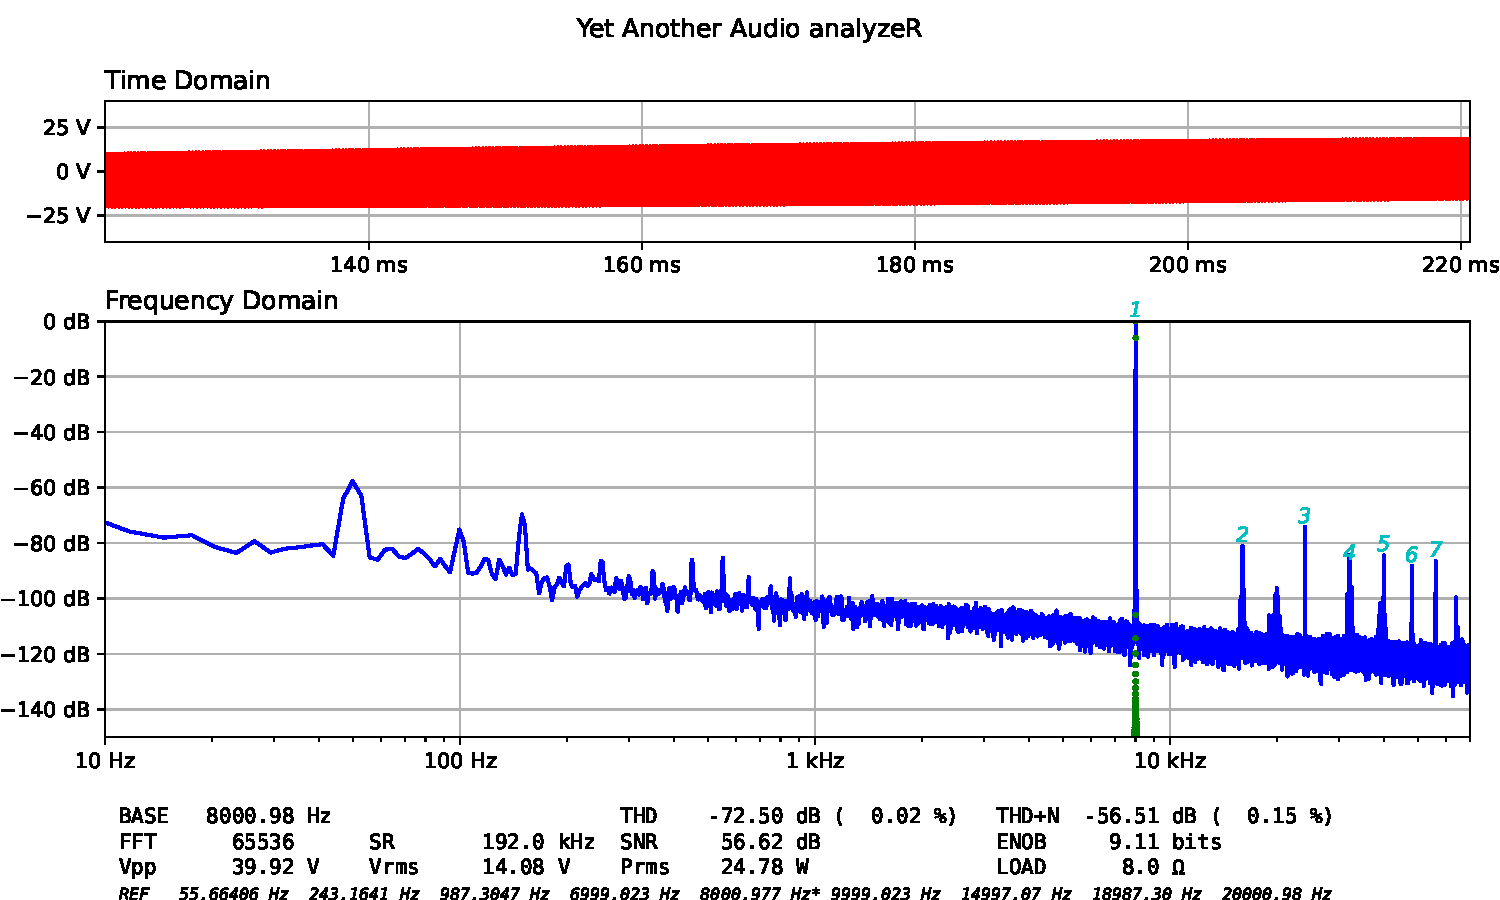
\includegraphics[width=0.95\textwidth]{measurements/yamaha_ca800ii_phono_right_8001Hz_0Hz.pdf}
    \caption{Right channel phono-stage THD measurement at 8.001\,kHz.}
\end{figure}

\begin{figure}[H]
    \centering
    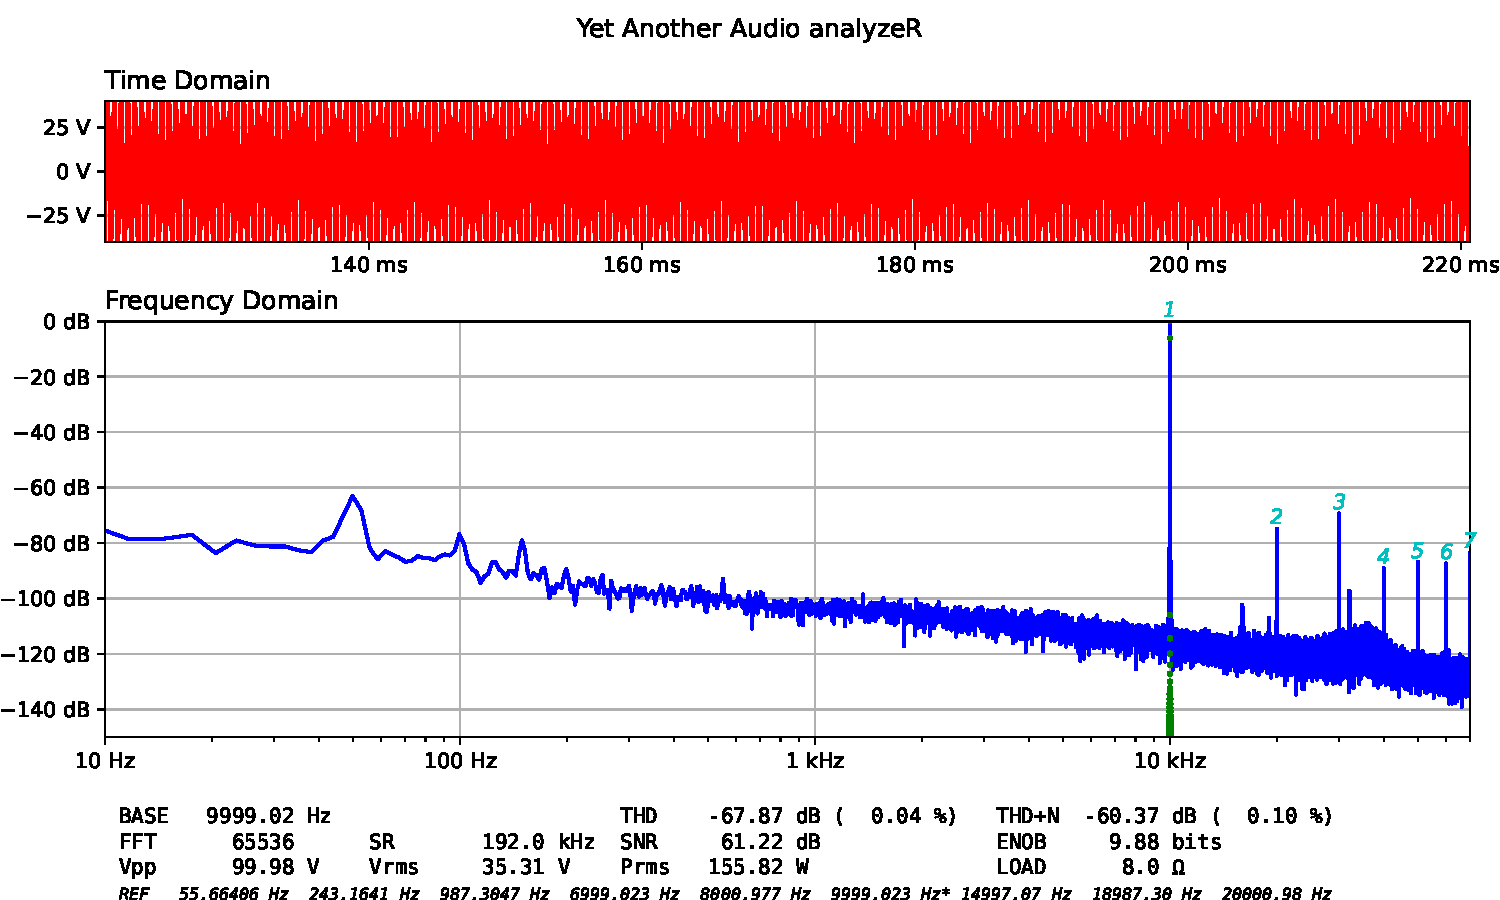
\includegraphics[width=0.95\textwidth]{measurements/yamaha_ca800ii_phono_right_9999Hz_0Hz.pdf}
    \caption{Right channel phono-stage THD measurement at 9.999\,kHz.}
\end{figure}

\begin{figure}[H]
    \centering
    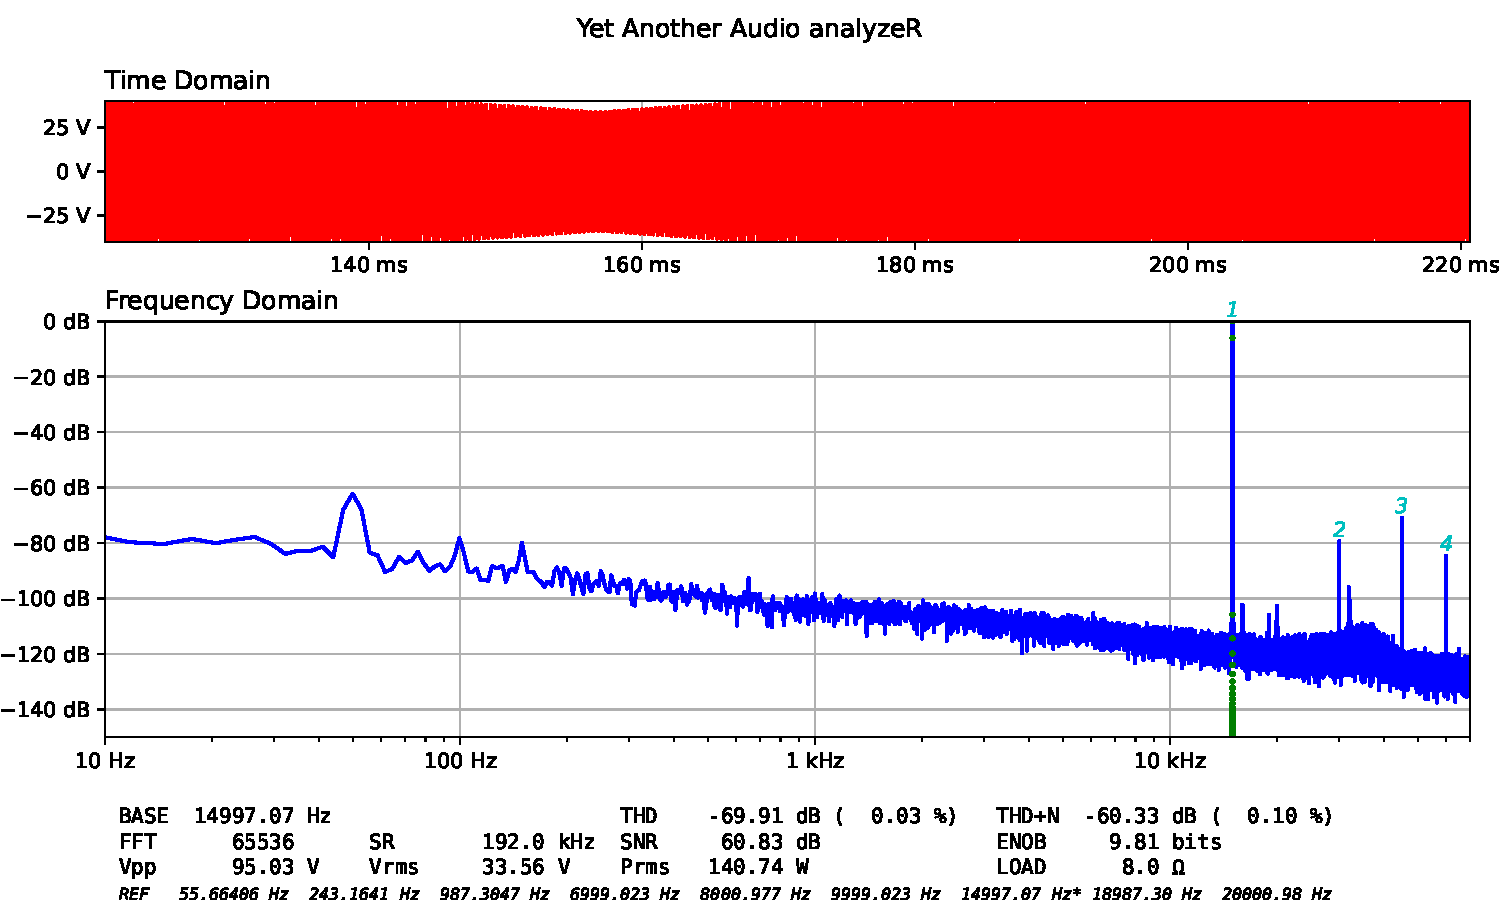
\includegraphics[width=0.95\textwidth]{measurements/yamaha_ca800ii_phono_right_14997Hz_0Hz.pdf}
    \caption{Right channel phono-stage THD measurement at 14.997\,kHz.}
\end{figure}

\begin{figure}[H]
    \centering
    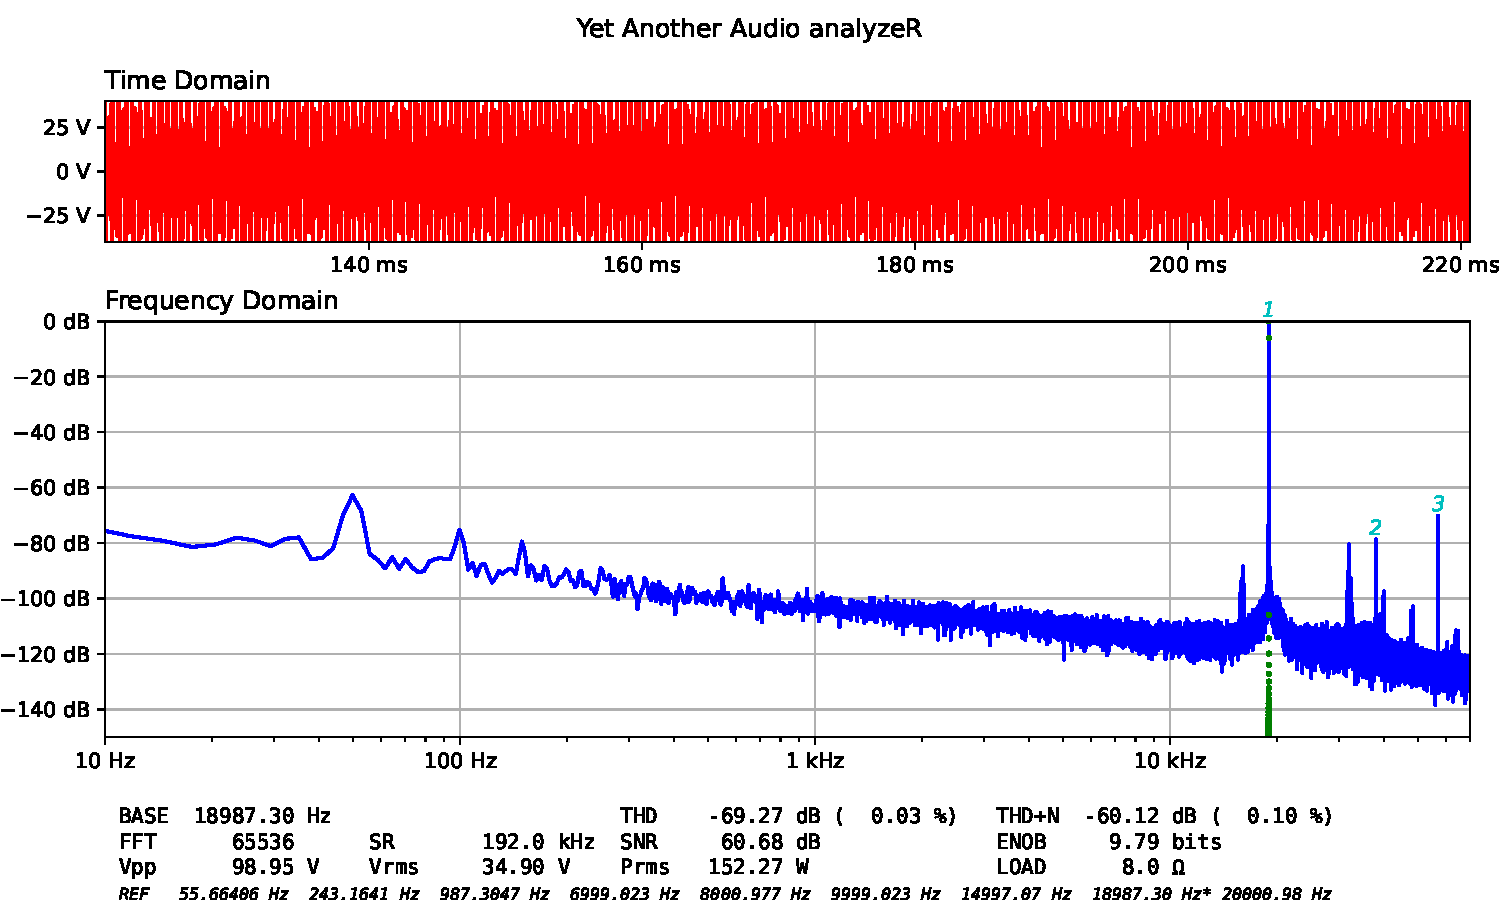
\includegraphics[width=0.95\textwidth]{measurements/yamaha_ca800ii_phono_right_18987Hz_0Hz.pdf}
    \caption{Right channel phono-stage THD measurement at 18.987\,kHz.}
\end{figure}

\begin{figure}[H]
    \centering
    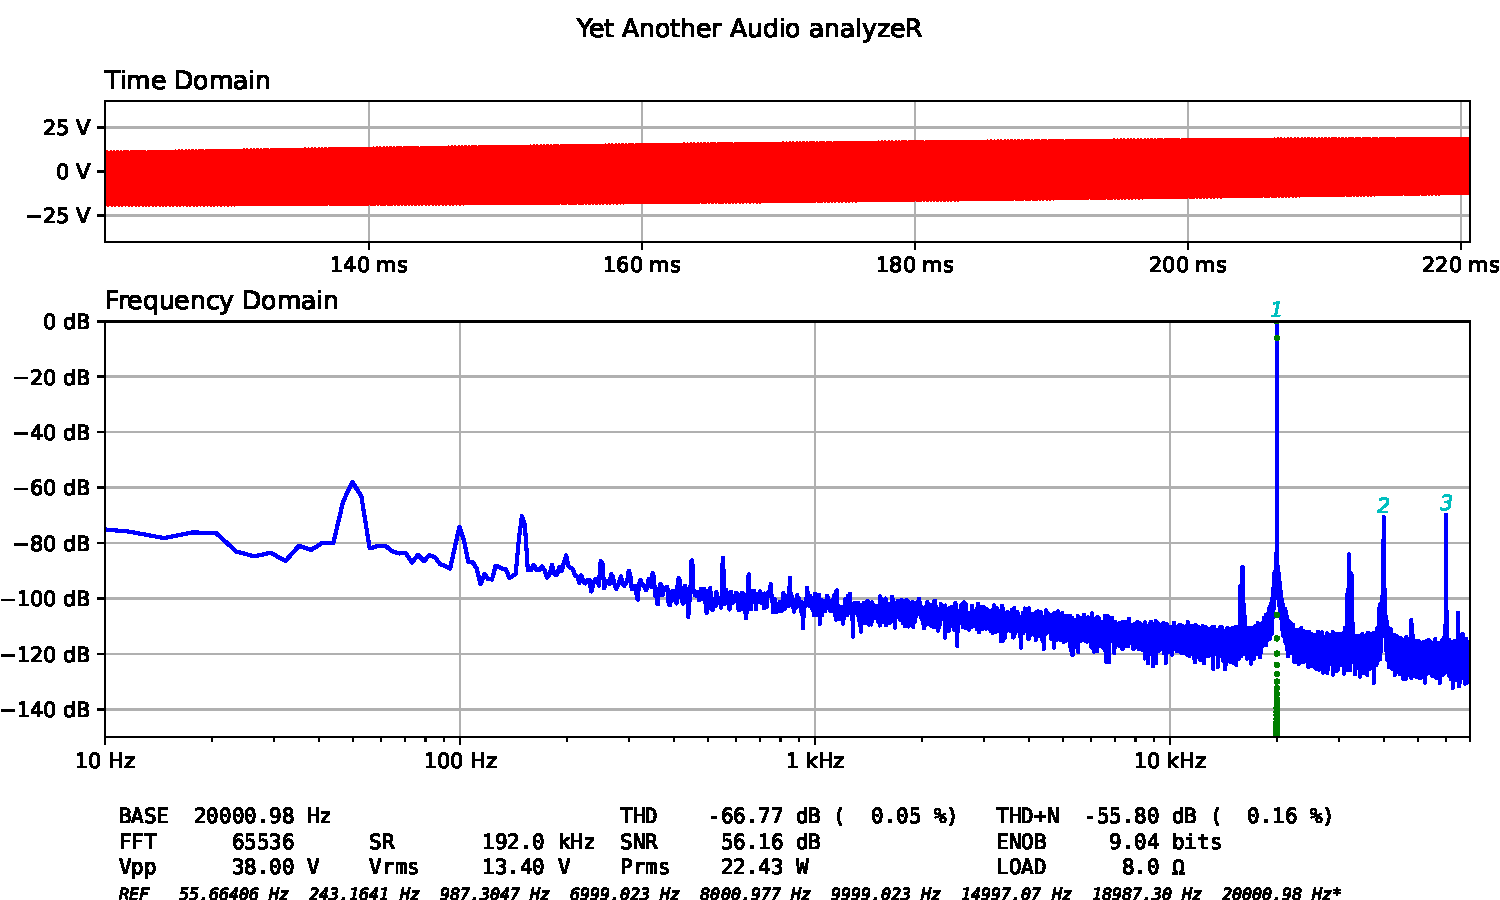
\includegraphics[width=0.95\textwidth]{measurements/yamaha_ca800ii_phono_right_20001Hz_0Hz.pdf}
    \caption{Right channel phono-stage THD measurement at 20.001\,kHz.}
\end{figure}

The right channel CCIF/SMPTE intermodulation measurement also demonstrates excellent high-frequency linearity and low intermodulation products after restoration.

\begin{figure}[H]
    \centering
    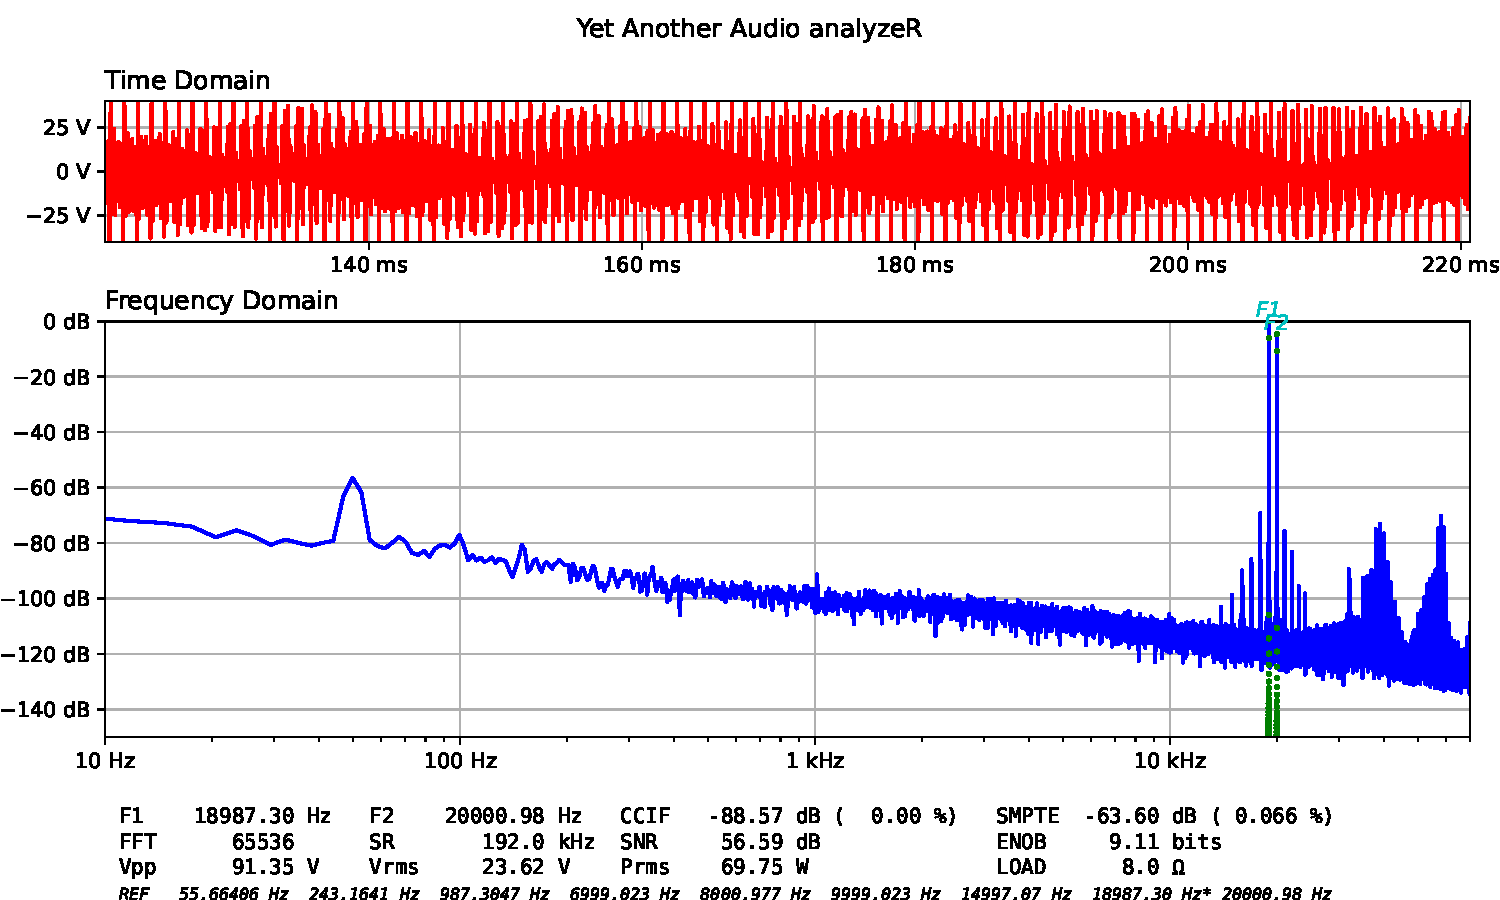
\includegraphics[width=0.95\textwidth]{measurements/yamaha_ca800ii_phono_right_18987Hz_20001Hz.pdf}
    \caption{Right channel phono-stage CCIF/SMPTE IMD measurement.}
\end{figure}

Overall, the phono-stage measurements confirm that the restoration successfully returned the Yamaha CA-800II equalizer and amplification stages to stable and low-distortion operation. Channel matching remains excellent, and the measured performance is fully consistent with a properly functioning high-quality vintage phono preamplifier and integrated amplifier design.

\subsection{Aux}

To evaluate the performance of the line-level input stage and power amplifier section, a low-distortion signal generator was connected to the AUX1 input of the Yamaha CA-800II. The generator output level was set to \(250\,\mathrm{mV}_{\mathrm{rms}}\). The amplifier outputs were terminated with non-inductive \(8\,\Omega\) load resistors, and the volume control was adjusted to produce approximately \(25\,\mathrm{W}\) output power. The same input level and volume setting were maintained throughout the measurement sequence.

Measurements were performed using Yet Another Audio Analyzer (YAAA) with a \(192\,\mathrm{kHz}\) sampling rate and \(65536\)-point FFT analysis. Both channels were characterized across the audio spectrum to evaluate total harmonic distortion (THD), THD+N, and intermodulation behavior after restoration.

The measurements show that both channels maintain consistently low distortion across most of the audible band, with THD typically remaining between \(0.04\%\) and \(0.06\%\). Harmonic content is dominated by low-order components, and no signs of instability or parasitic oscillation were observed during high-frequency testing.

\subsubsection{Left Channel}

At low frequencies, the left channel exhibits very clean sinusoidal behavior with low harmonic distortion and a stable noise floor.

\begin{figure}[H]
	\centering
	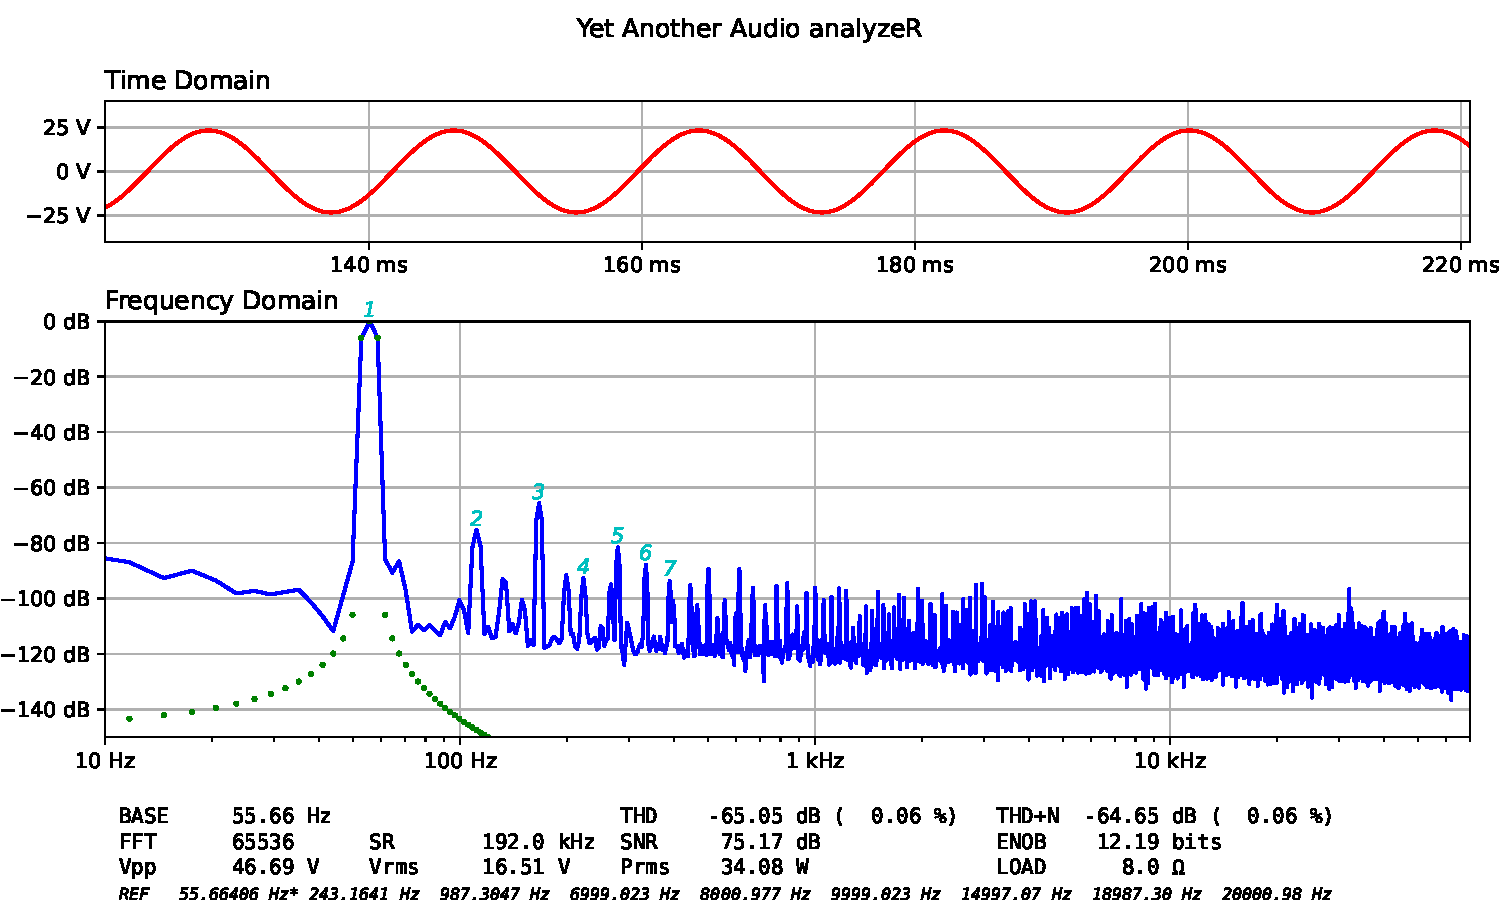
\includegraphics[width=\linewidth]{measurements/yamaha_ca800ii_aux_left_56Hz_0Hz.pdf}
	\caption{Left channel THD measurement at 55.66\,Hz.}
	\label{fig:aux_left_56hz}
\end{figure}

\begin{figure}[H]
	\centering
	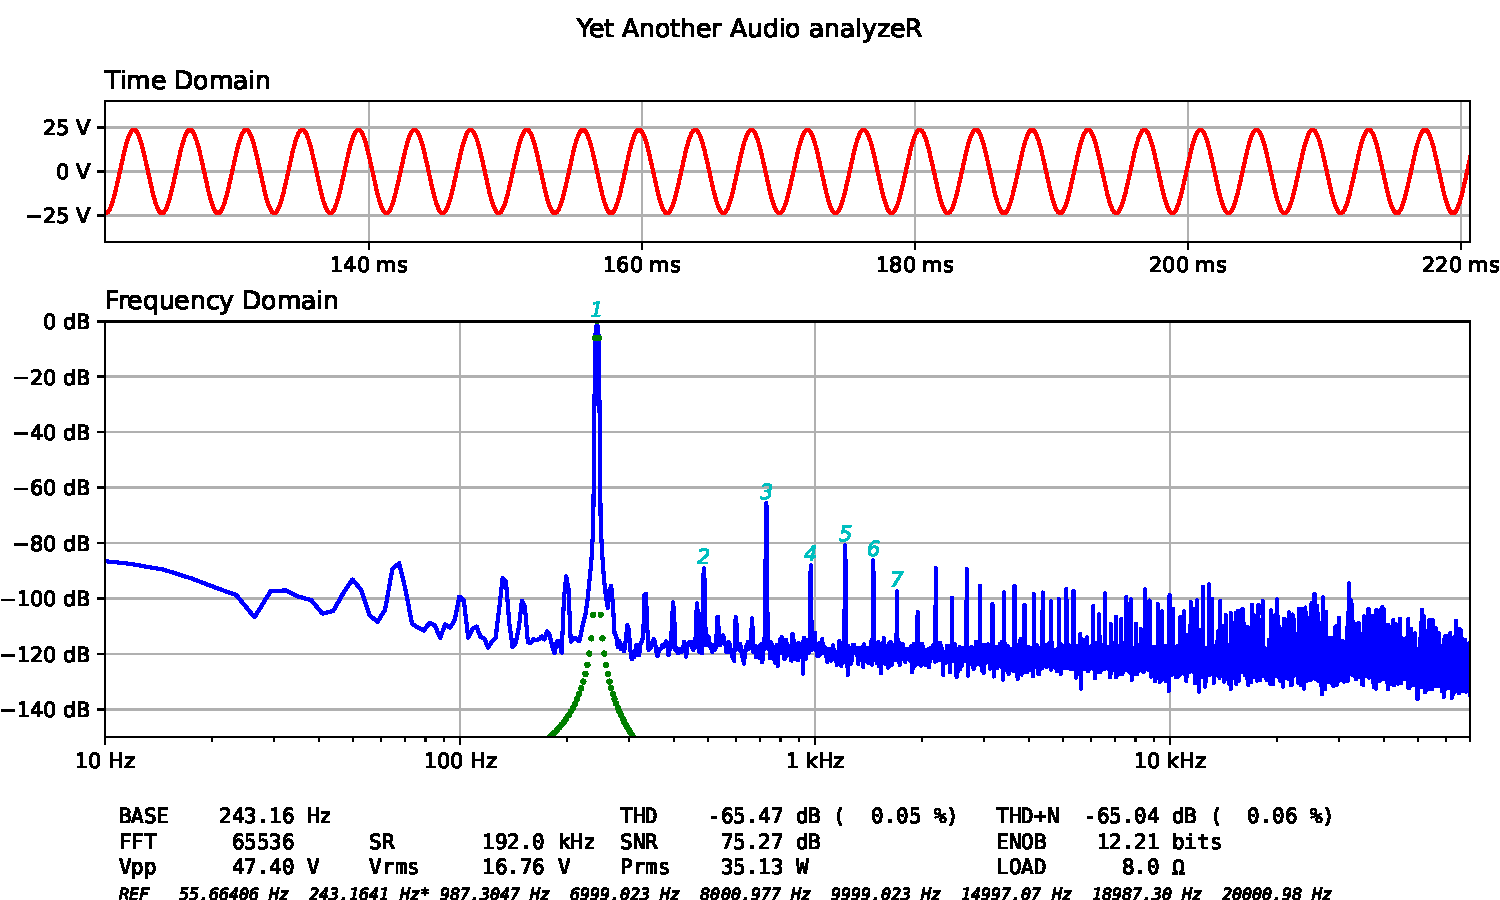
\includegraphics[width=\linewidth]{measurements/yamaha_ca800ii_aux_left_243Hz_0Hz.pdf}
	\caption{Left channel THD measurement at 243.16\,Hz.}
	\label{fig:aux_left_243hz}
\end{figure}

Midband performance remains essentially unchanged, indicating good linearity through the voltage amplification and driver stages.

\begin{figure}[H]
	\centering
	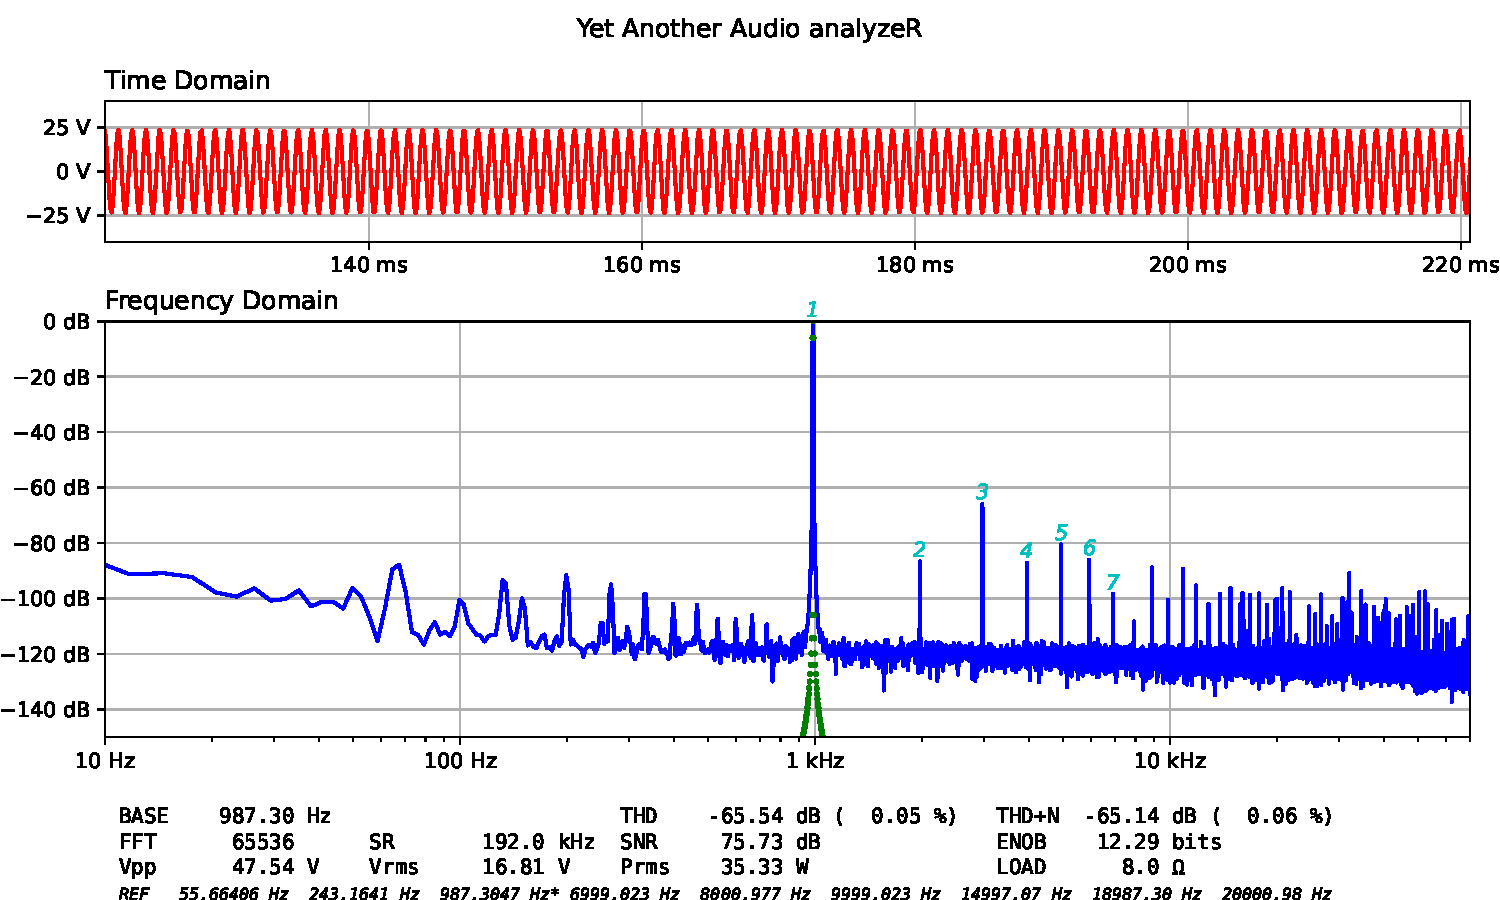
\includegraphics[width=\linewidth]{measurements/yamaha_ca800ii_aux_left_987Hz_0Hz.pdf}
	\caption{Left channel THD measurement at 987.30\,Hz.}
	\label{fig:aux_left_1khz}
\end{figure}

At higher frequencies, a gradual rise in high-order harmonic content and broadband noise becomes visible, though distortion remains low overall.

\begin{figure}[H]
	\centering
	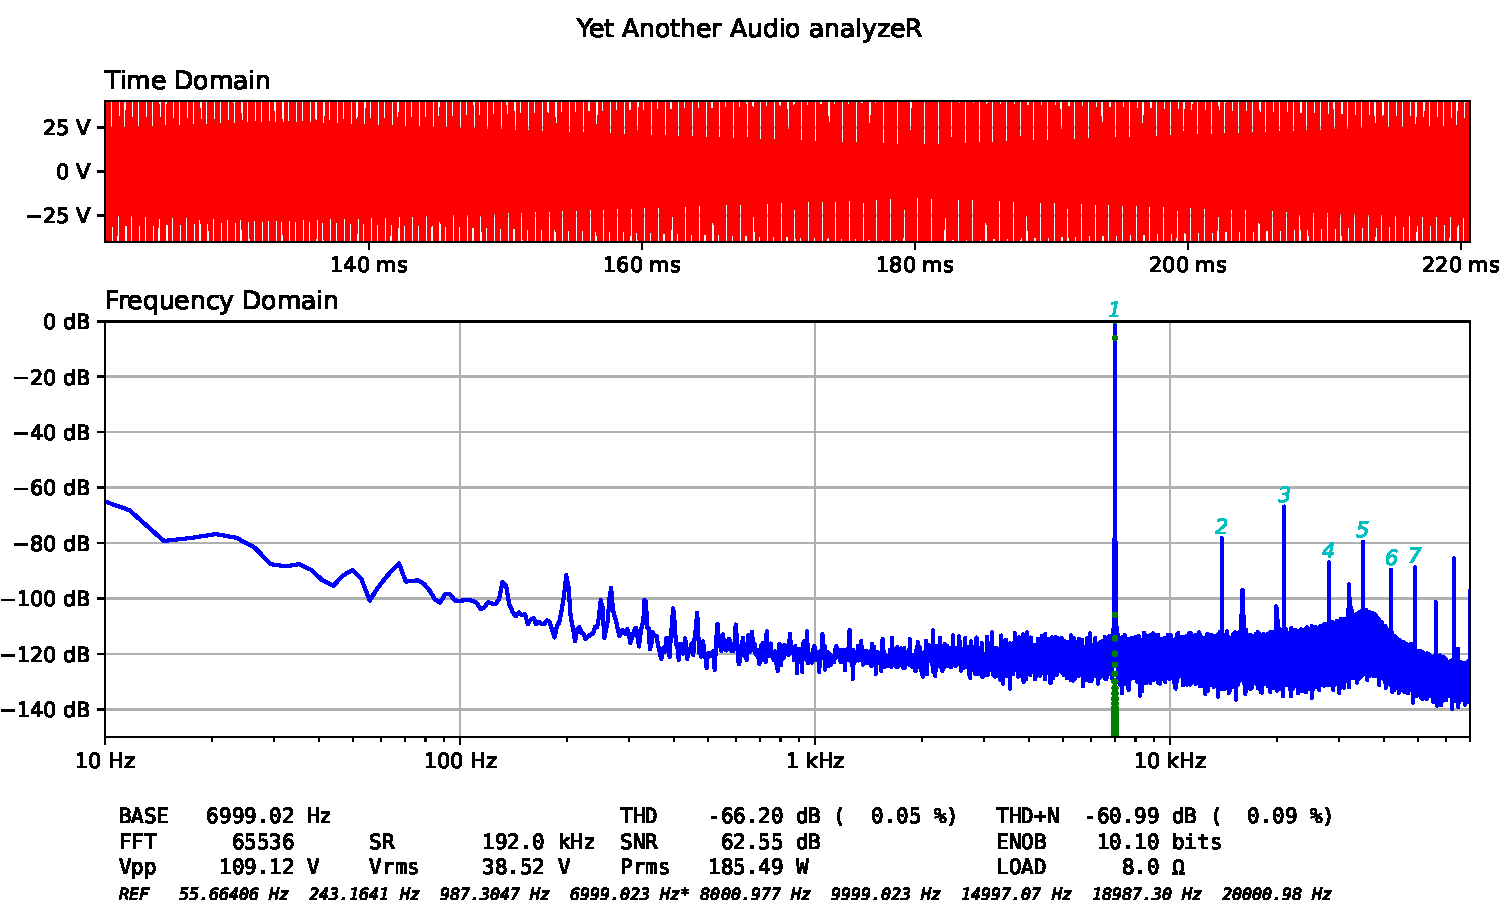
\includegraphics[width=\linewidth]{measurements/yamaha_ca800ii_aux_left_6999Hz_0Hz.pdf}
	\caption{Left channel THD measurement at 6.999\,kHz.}
	\label{fig:aux_left_7khz}
\end{figure}

\begin{figure}[H]
	\centering
	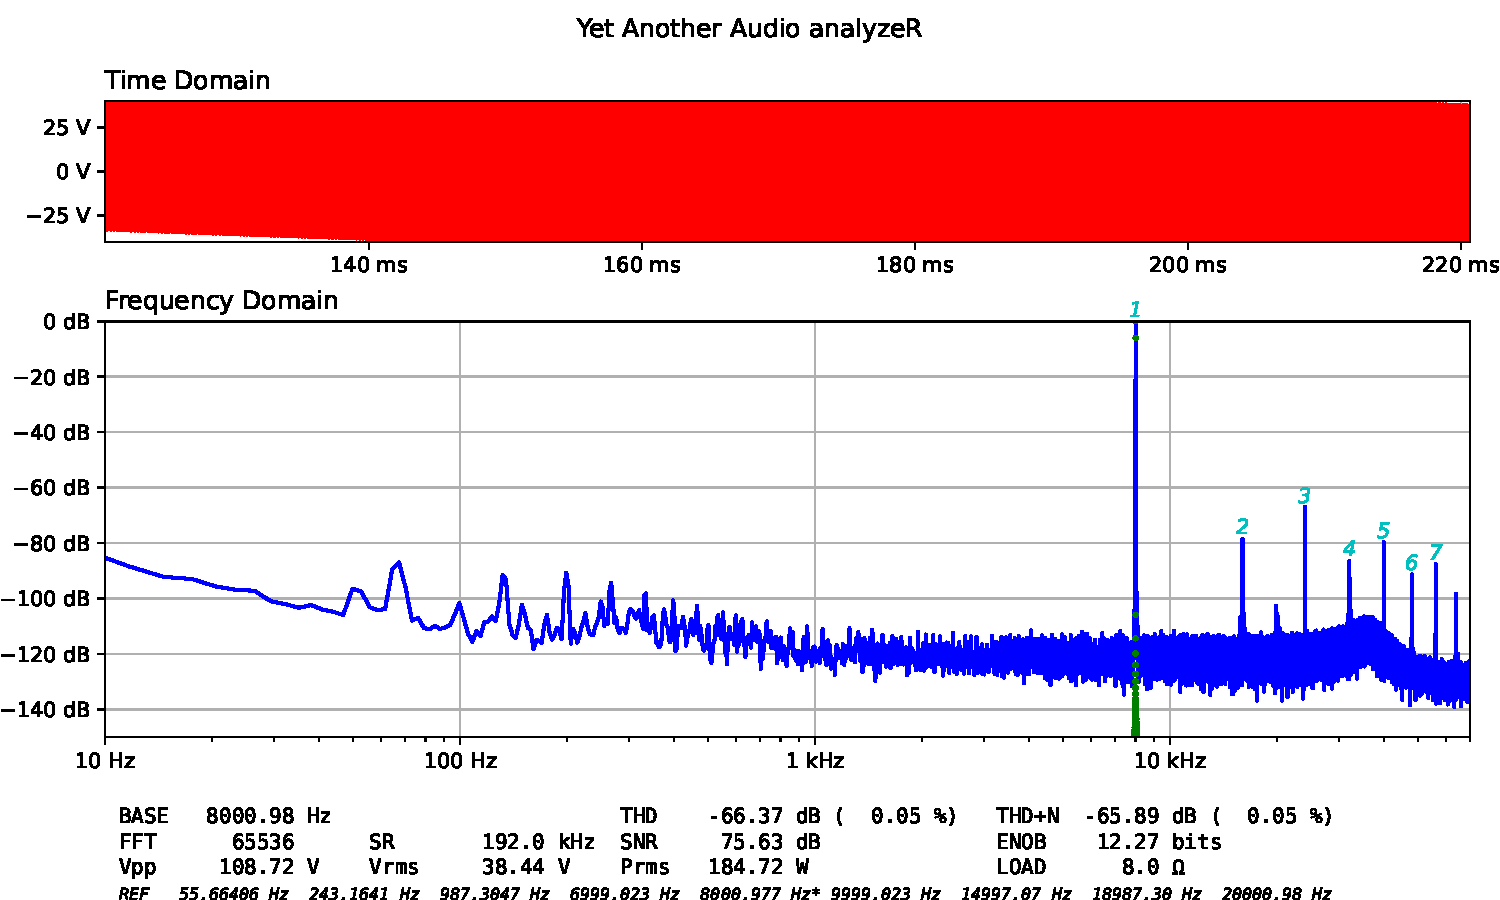
\includegraphics[width=\linewidth]{measurements/yamaha_ca800ii_aux_left_8001Hz_0Hz.pdf}
	\caption{Left channel THD measurement at 8.001\,kHz.}
	\label{fig:aux_left_8khz}
\end{figure}

\begin{figure}[H]
	\centering
	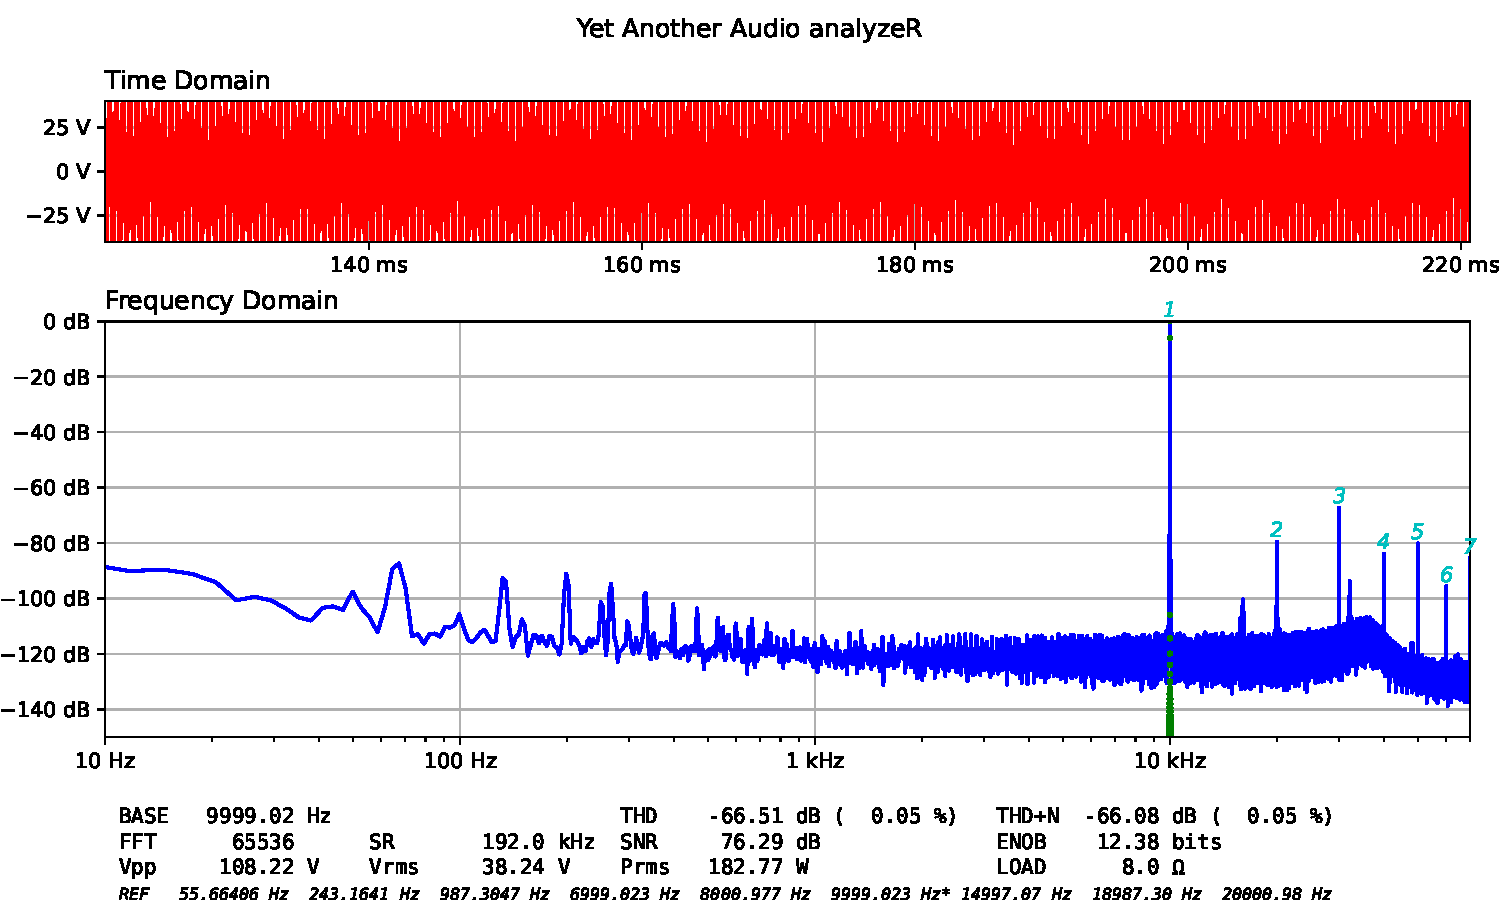
\includegraphics[width=\linewidth]{measurements/yamaha_ca800ii_aux_left_9999Hz_0Hz.pdf}
	\caption{Left channel THD measurement at 9.999\,kHz.}
	\label{fig:aux_left_10khz}
\end{figure}

\begin{figure}[H]
	\centering
	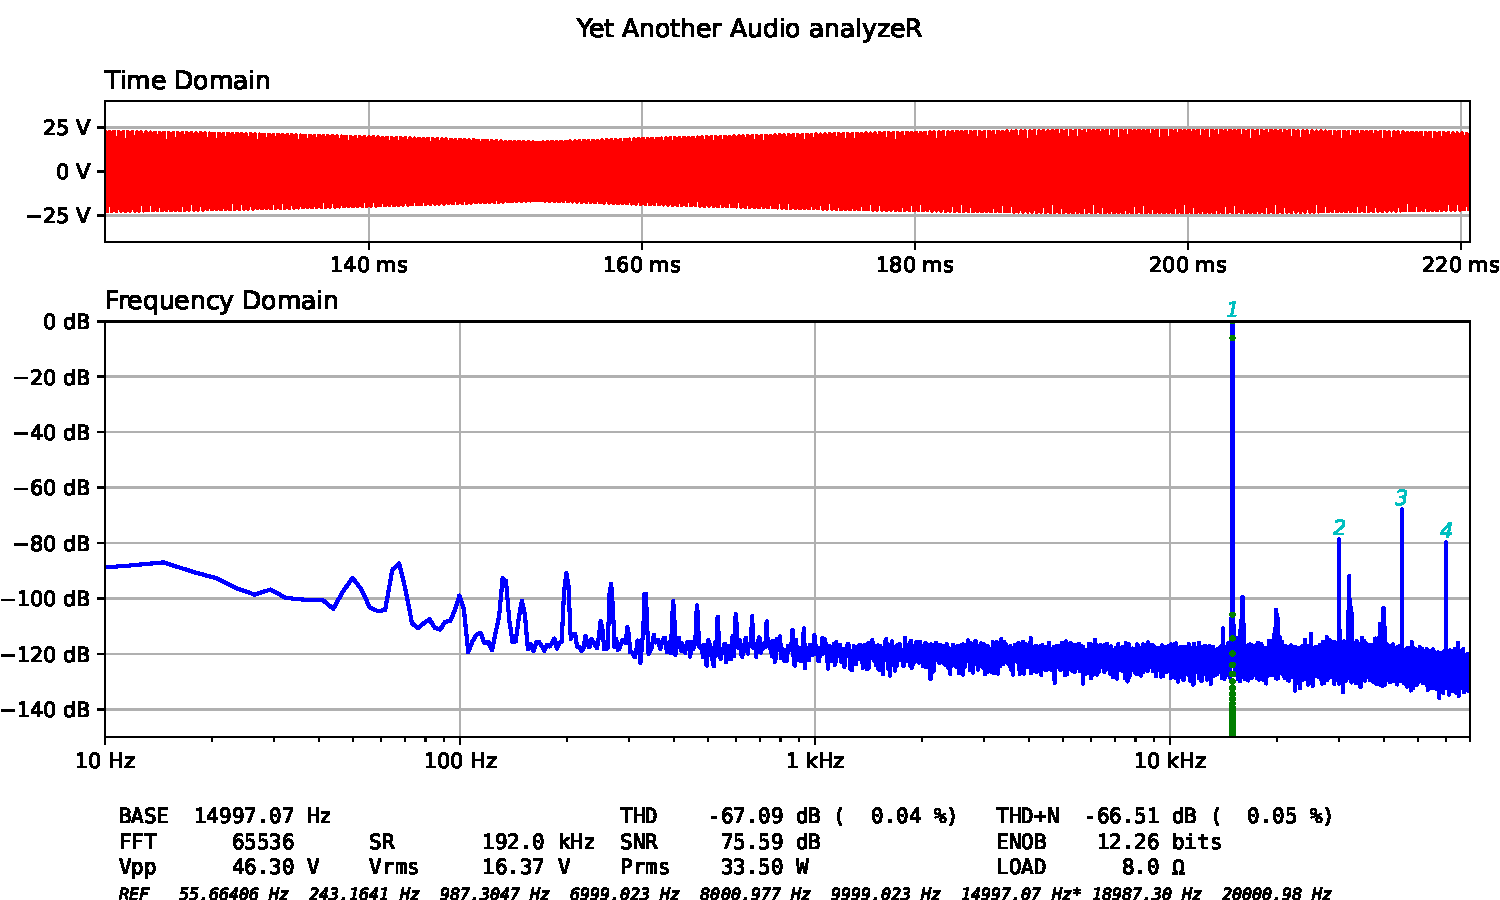
\includegraphics[width=\linewidth]{measurements/yamaha_ca800ii_aux_left_14997Hz_0Hz.pdf}
	\caption{Left channel THD measurement at 14.997\,kHz.}
	\label{fig:aux_left_15khz}
\end{figure}

\begin{figure}[H]
	\centering
	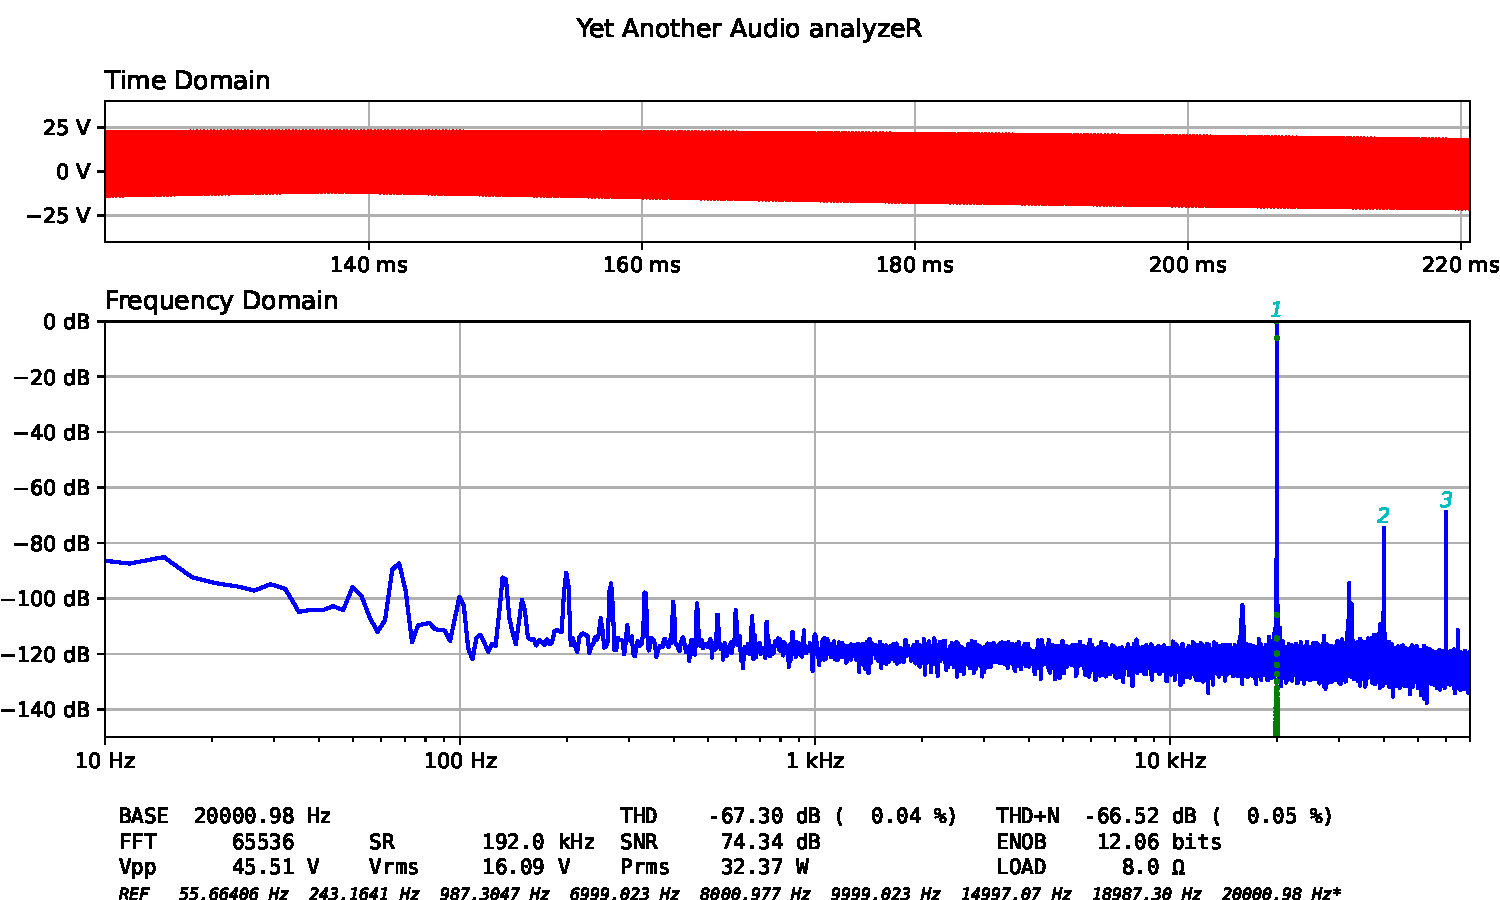
\includegraphics[width=\linewidth]{measurements/yamaha_ca800ii_aux_left_20001Hz_0Hz.pdf}
	\caption{Left channel THD measurement at 20.001\,kHz.}
	\label{fig:aux_left_20khz}
\end{figure}

A CCIF intermodulation test was also performed using 18.987\,kHz and 20.001\,kHz twin tones. The resulting spectrum demonstrates excellent stability and very low intermodulation products.

\begin{figure}[H]
	\centering
	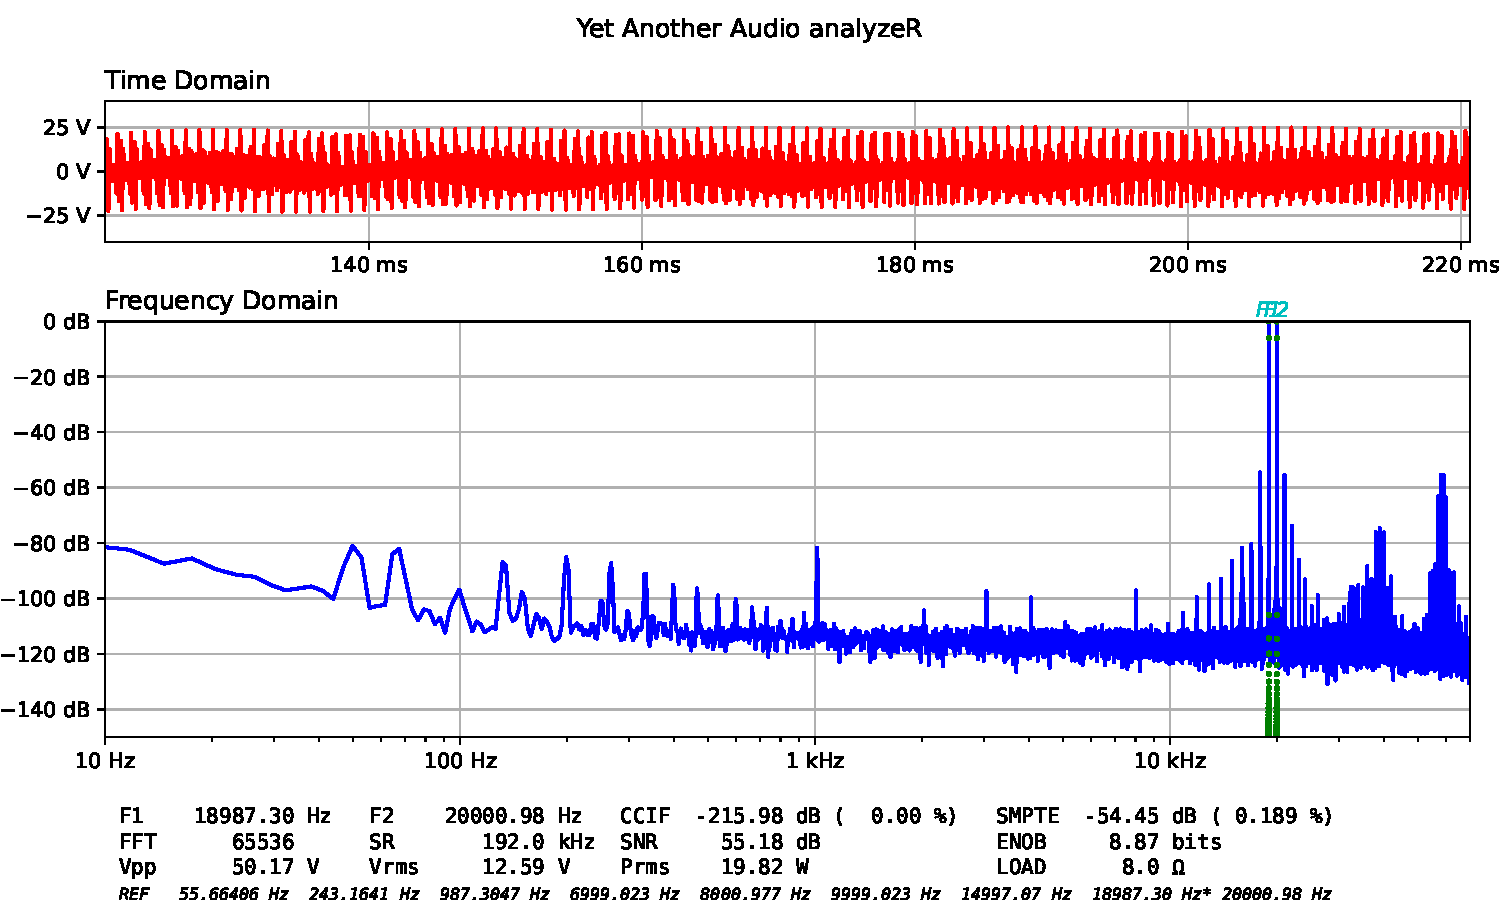
\includegraphics[width=\linewidth]{measurements/yamaha_ca800ii_aux_left_18987Hz_20001Hz.pdf}
	\caption{Left channel CCIF/SMPTE intermodulation distortion measurement.}
	\label{fig:aux_left_imd}
\end{figure}

\subsubsection{Right Channel}

The right channel measurements closely track the behavior of the left channel, with similarly low harmonic distortion and clean spectral performance.

\begin{figure}[H]
	\centering
	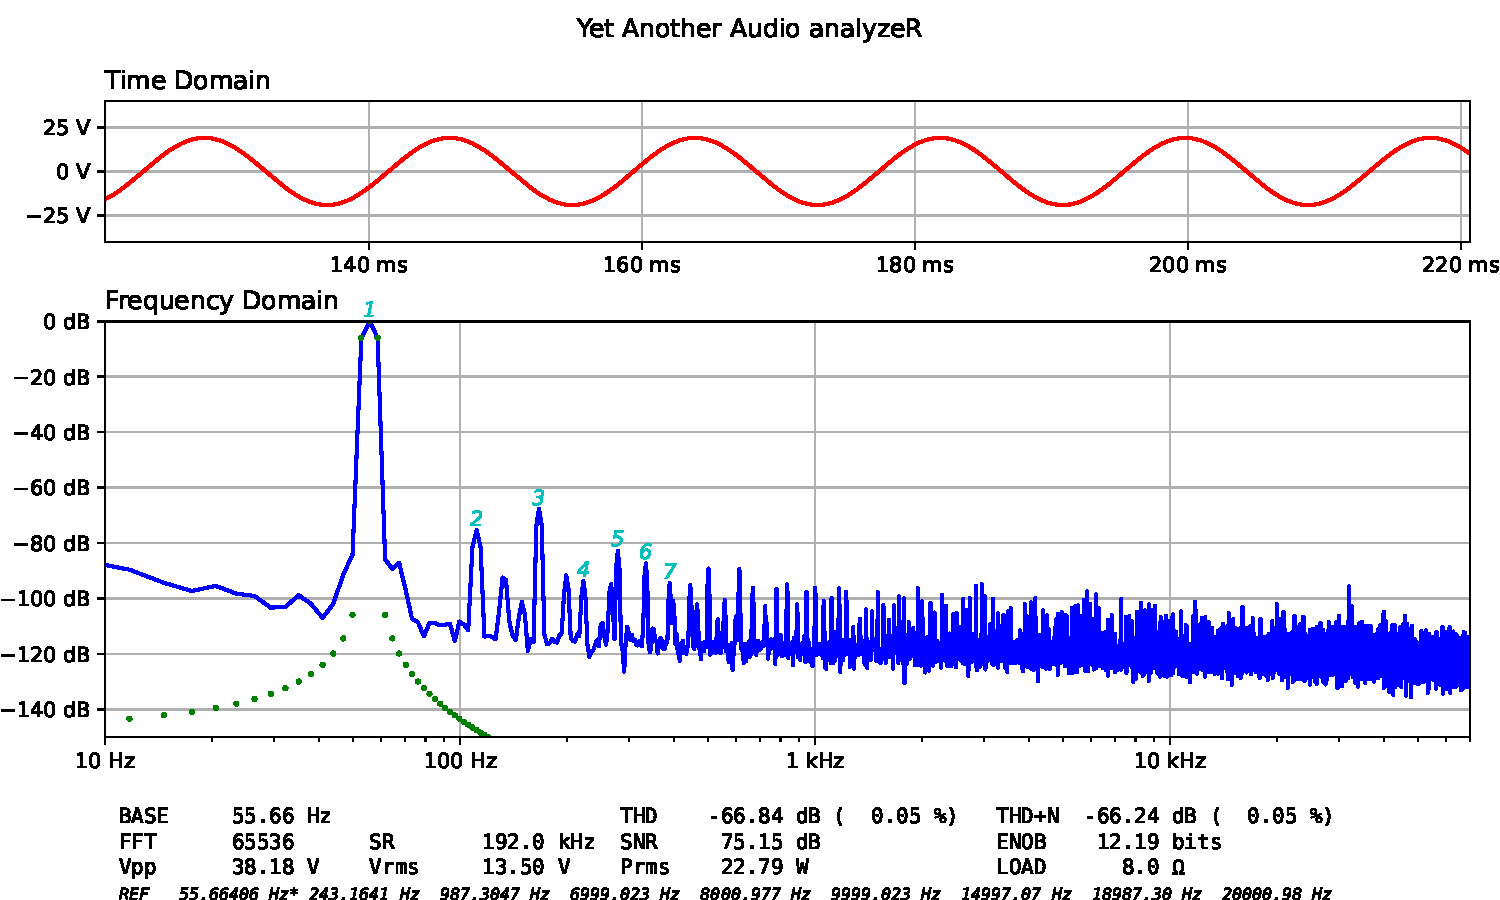
\includegraphics[width=\linewidth]{measurements/yamaha_ca800ii_aux_right_56Hz_0Hz.pdf}
	\caption{Right channel THD measurement at 55.66\,Hz.}
	\label{fig:aux_right_56hz}
\end{figure}

\begin{figure}[H]
	\centering
	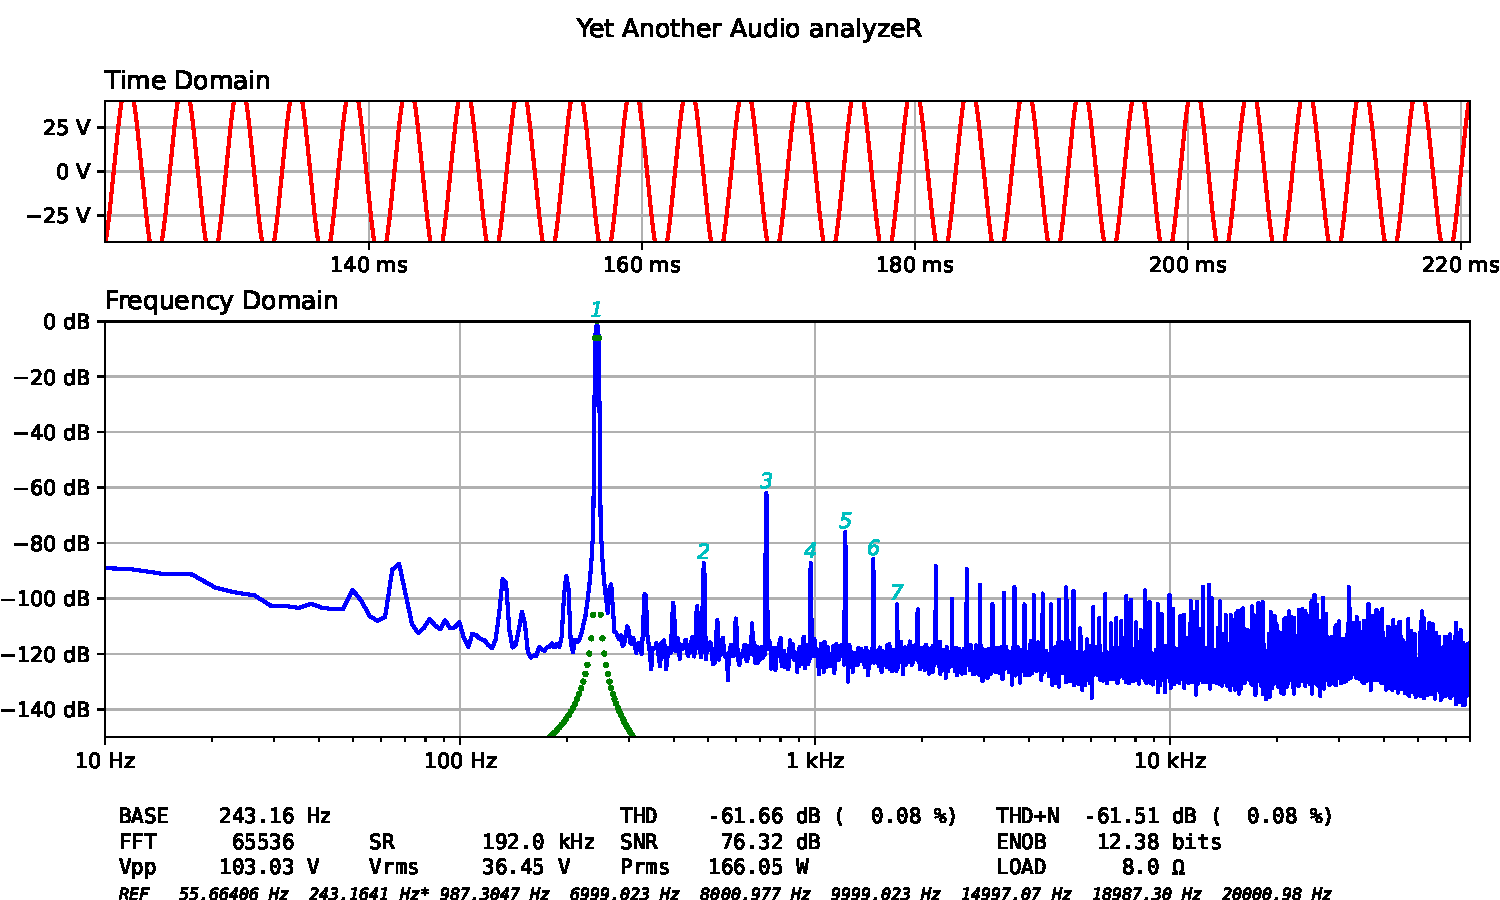
\includegraphics[width=\linewidth]{measurements/yamaha_ca800ii_aux_right_243Hz_0Hz.pdf}
	\caption{Right channel THD measurement at 243.16\,Hz.}
	\label{fig:aux_right_243hz}
\end{figure}

\begin{figure}[H]
	\centering
	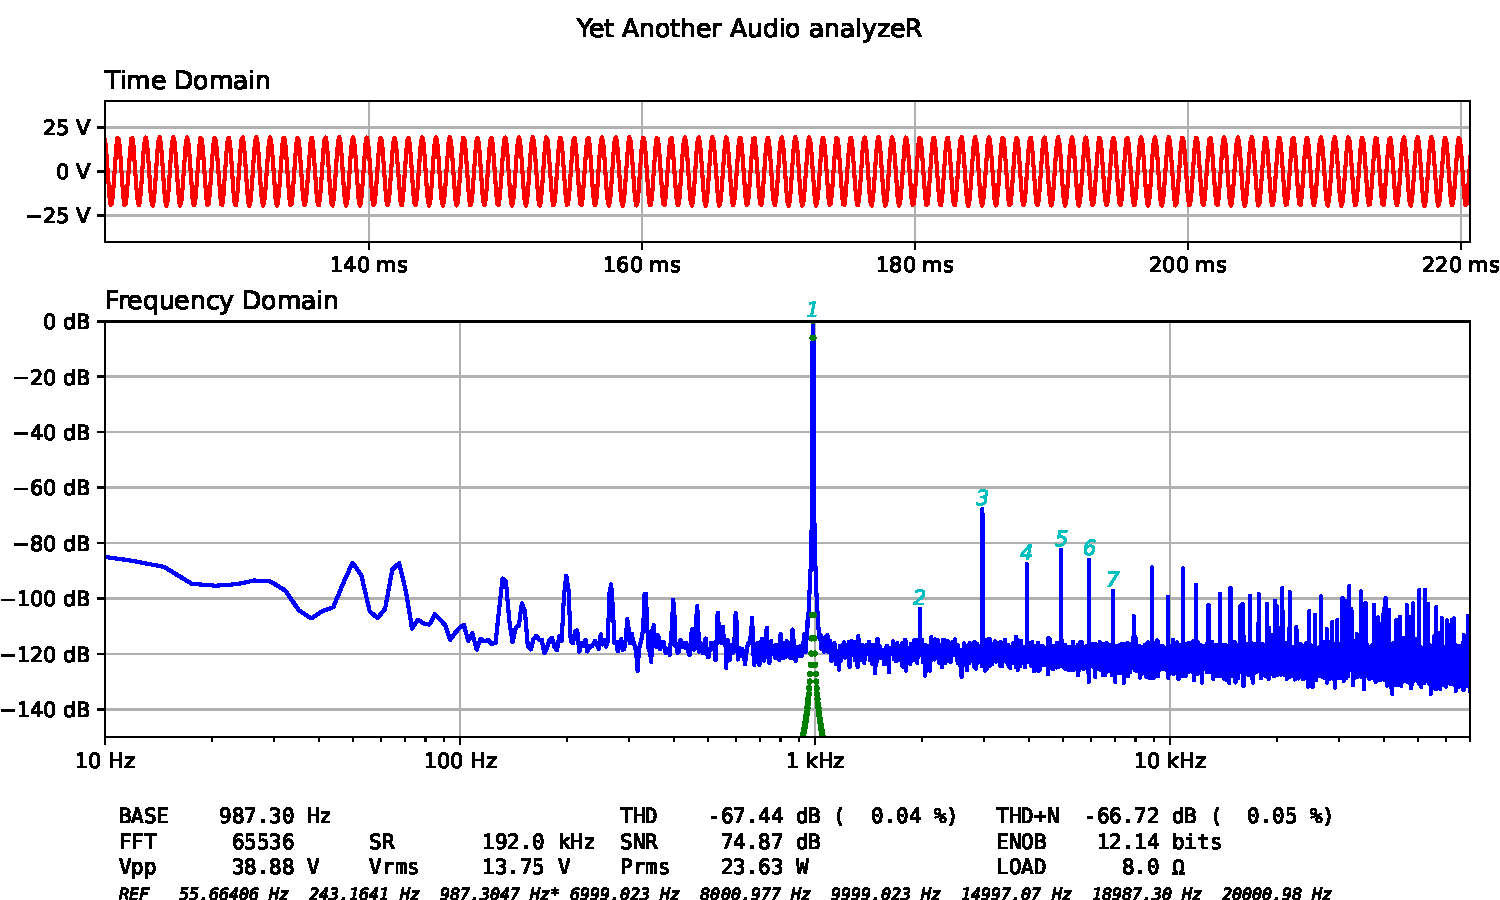
\includegraphics[width=\linewidth]{measurements/yamaha_ca800ii_aux_right_987Hz_0Hz.pdf}
	\caption{Right channel THD measurement at 987.30\,Hz.}
	\label{fig:aux_right_1khz}
\end{figure}

High-frequency measurements indicate a moderate increase in THD+N above 10\,kHz, though overall amplifier behavior remains stable and well controlled.

\begin{figure}[H]
	\centering
	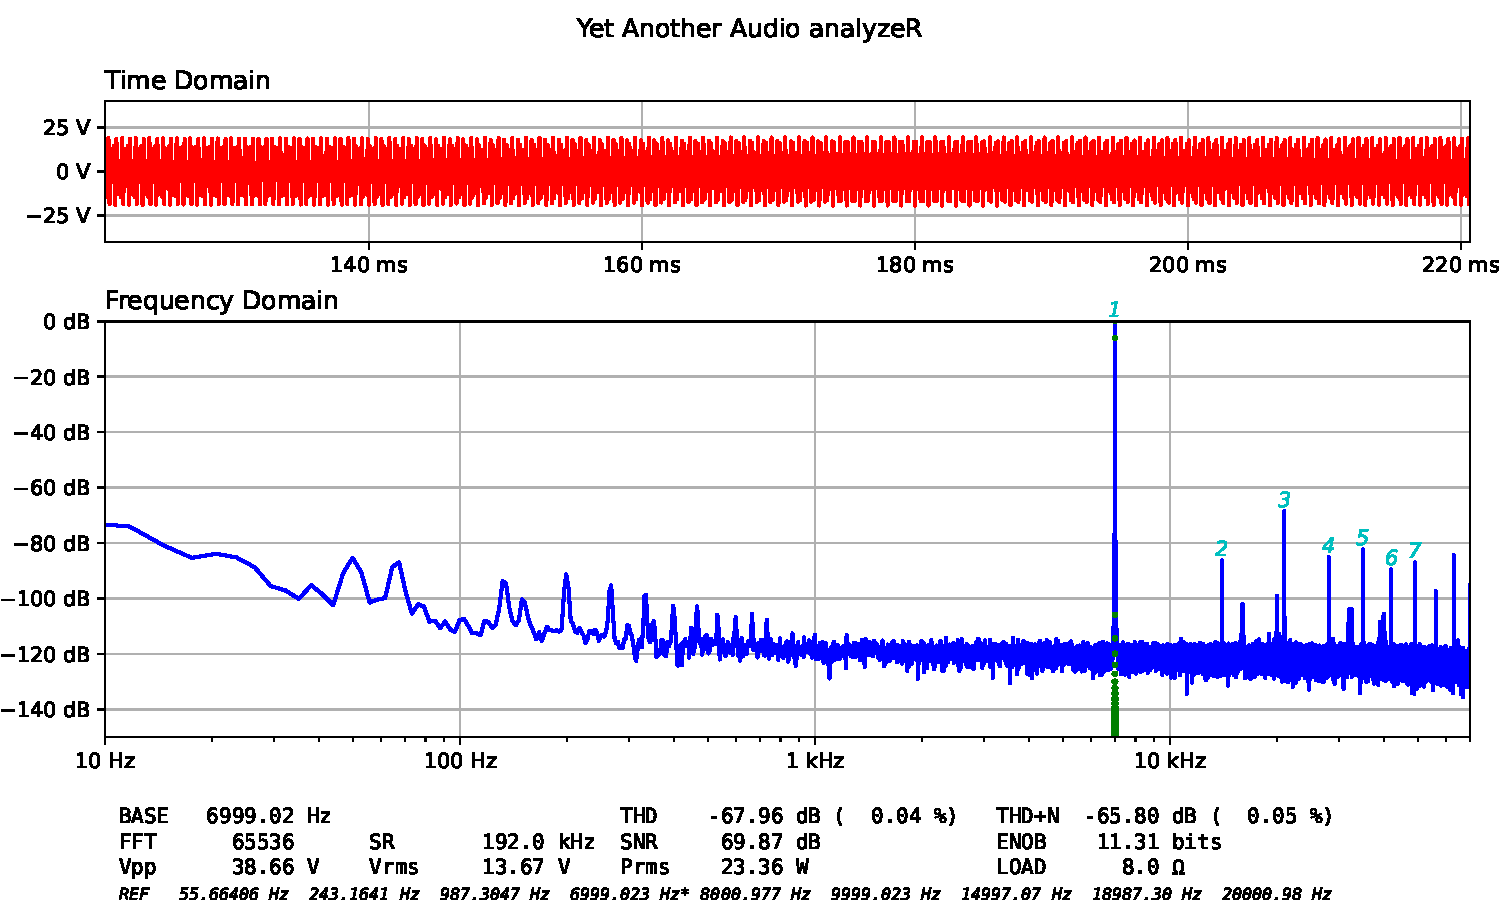
\includegraphics[width=\linewidth]{measurements/yamaha_ca800ii_aux_right_6999Hz_0Hz.pdf}
	\caption{Right channel THD measurement at 6.999\,kHz.}
	\label{fig:aux_right_7khz}
\end{figure}

\begin{figure}[H]
	\centering
	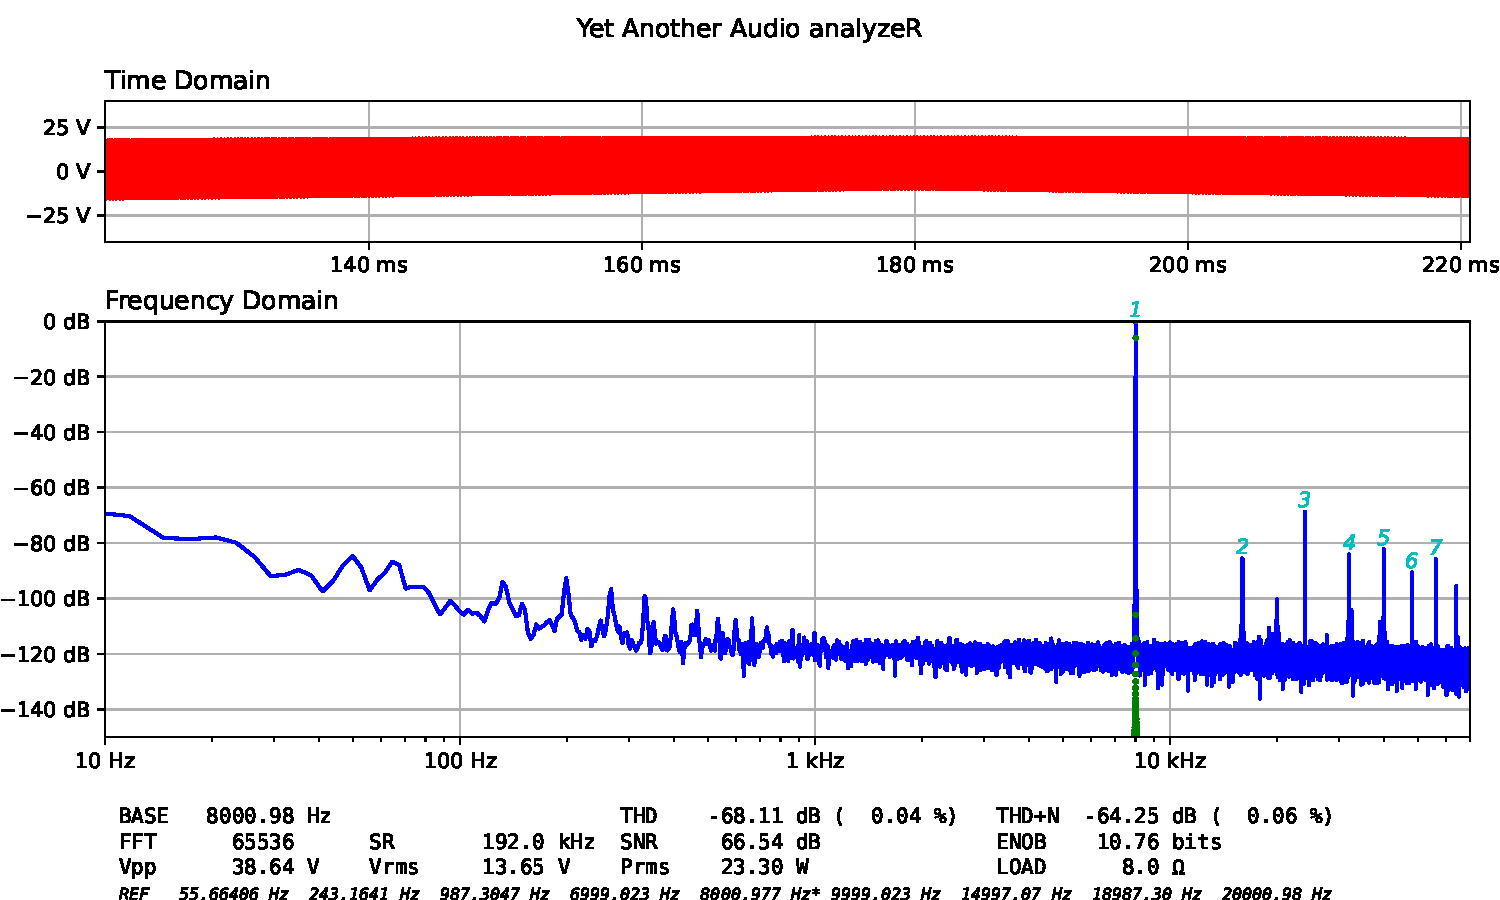
\includegraphics[width=\linewidth]{measurements/yamaha_ca800ii_aux_right_8001Hz_0Hz.pdf}
	\caption{Right channel THD measurement at 8.001\,kHz.}
	\label{fig:aux_right_8khz}
\end{figure}

\begin{figure}[H]
	\centering
	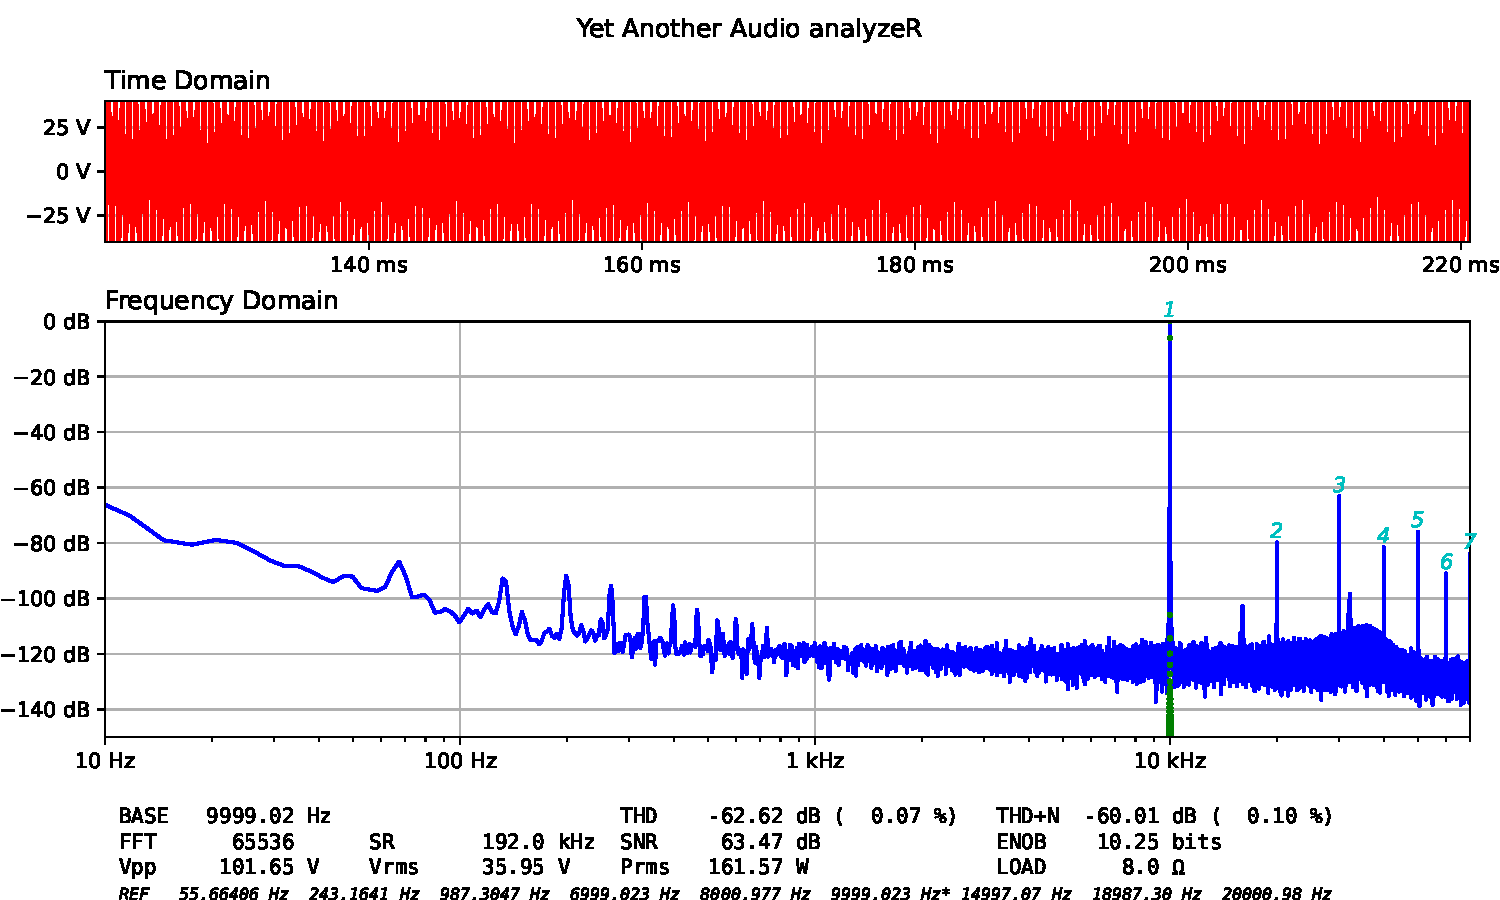
\includegraphics[width=\linewidth]{measurements/yamaha_ca800ii_aux_right_9999Hz_0Hz.pdf}
	\caption{Right channel THD measurement at 9.999\,kHz.}
	\label{fig:aux_right_10khz}
\end{figure}

\begin{figure}[H]
	\centering
	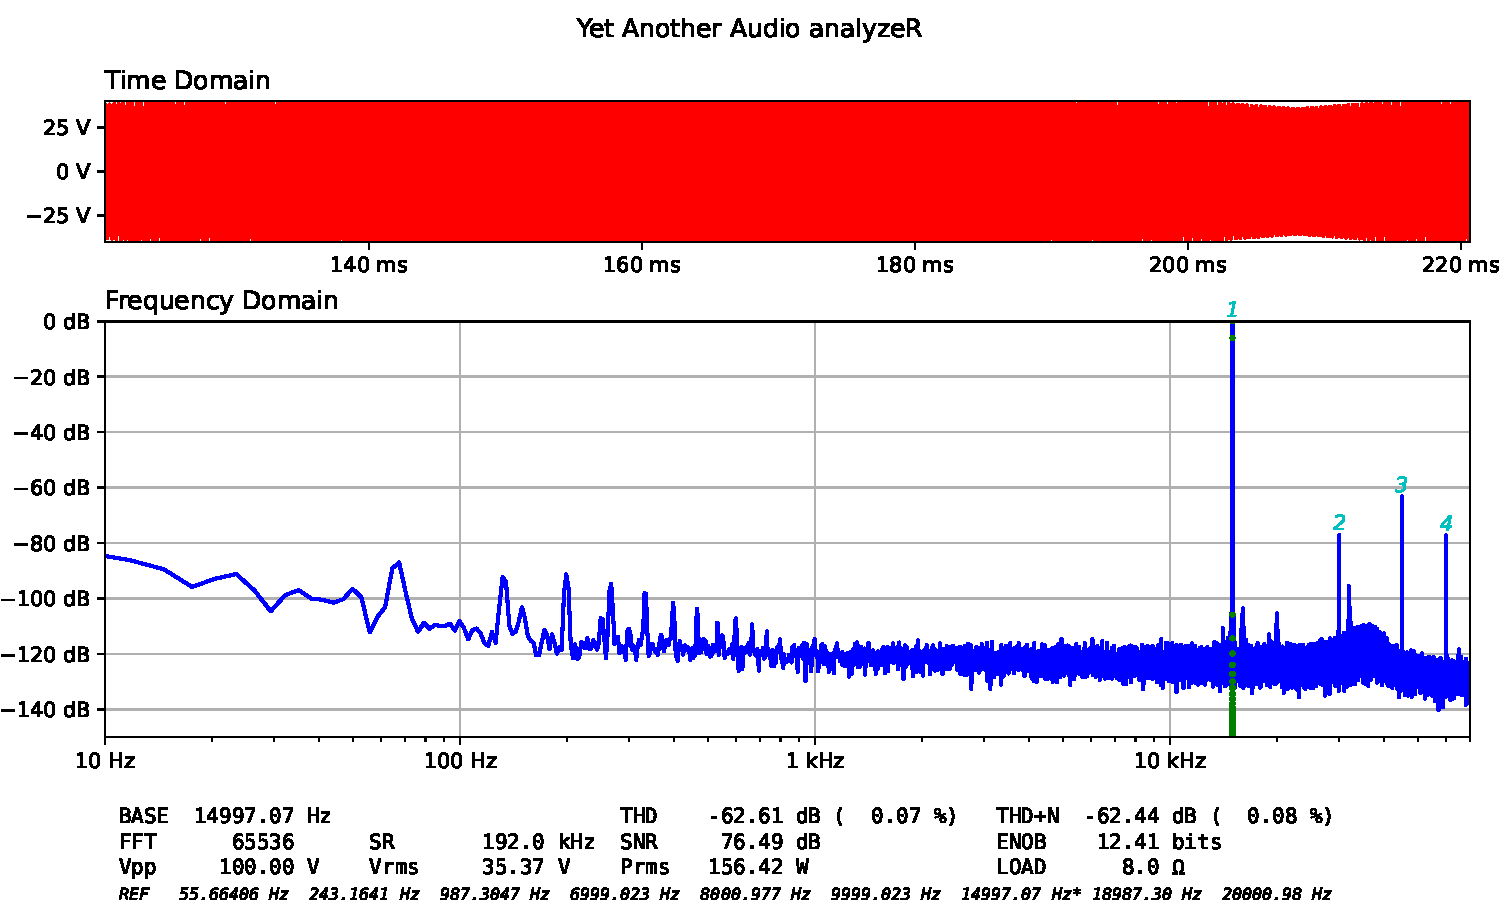
\includegraphics[width=\linewidth]{measurements/yamaha_ca800ii_aux_right_14997Hz_0Hz.pdf}
	\caption{Right channel THD measurement at 14.997\,kHz.}
	\label{fig:aux_right_15khz}
\end{figure}

The right channel intermodulation measurement also demonstrates excellent recovery after renovation, with very low CCIF distortion products and clean separation of the twin-tone carriers.

\begin{figure}[H]
	\centering
	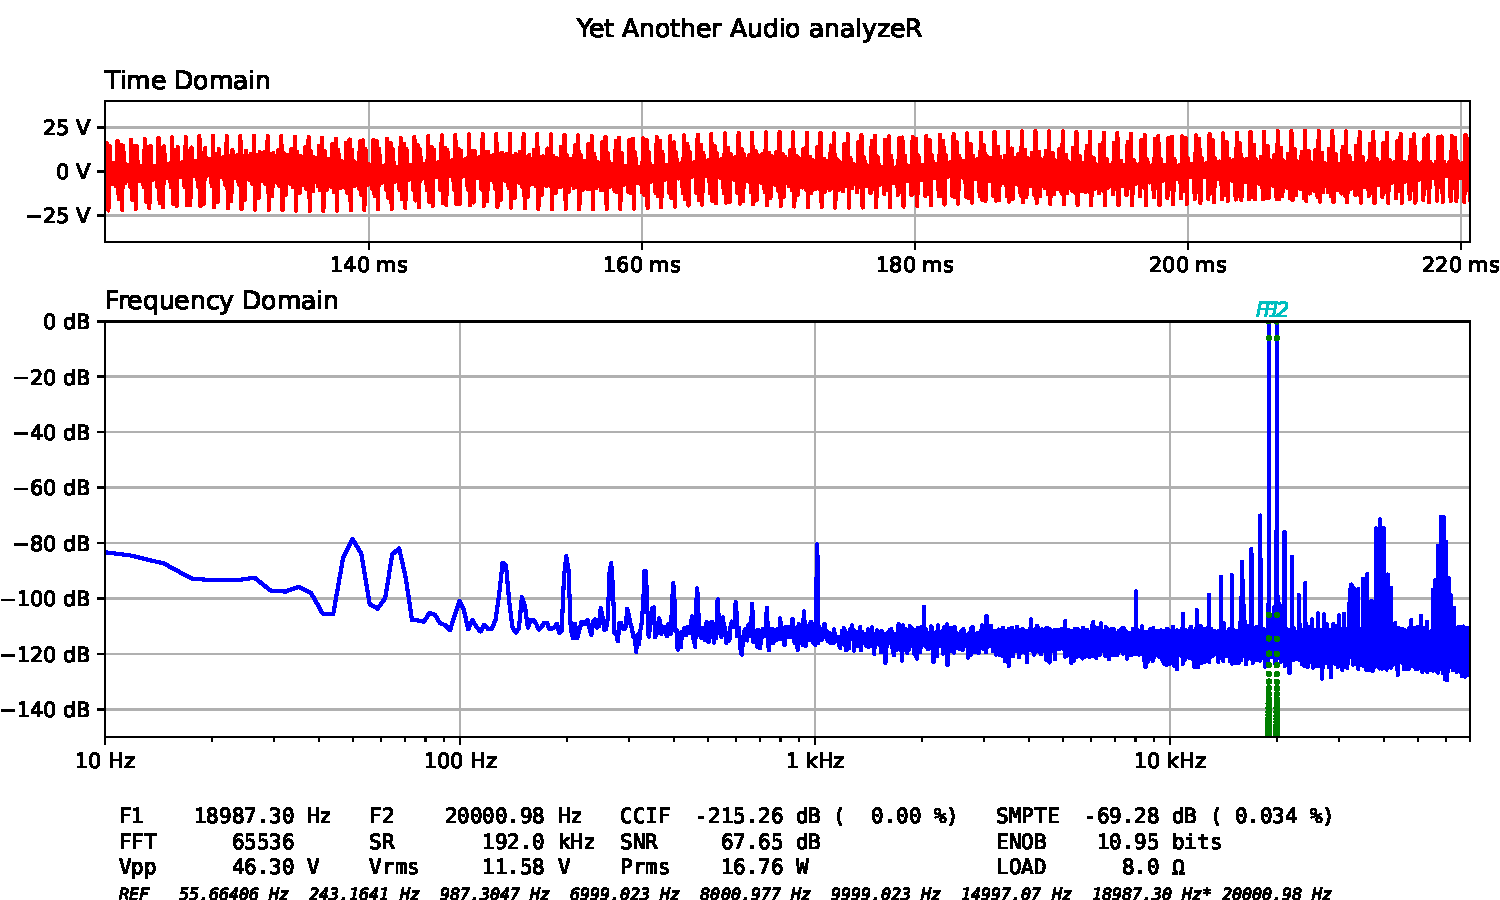
\includegraphics[width=\linewidth]{measurements/yamaha_ca800ii_aux_right_18987Hz_20001Hz.pdf}
	\caption{Right channel CCIF/SMPTE intermodulation distortion measurement.}
	\label{fig:aux_right_imd}
\end{figure}

Overall, the AUX input measurements confirm that the restoration work successfully returned the Yamaha CA-800II to stable and low-distortion operation. Both channels remain closely matched and exhibit performance consistent with a properly functioning high-quality vintage integrated amplifier.

\section{Appendix I: Phone NGSpice simulation}

\begin{verbatim}
* File: ACsim.cir
.title ACsim
.include mymodel.cir
.include include.cir

V1 SUP 0 51 
V2 IN 0 AC 0.004
RLoad OUT 0 47k
Rleak_IN IN 0 100Meg 
Rleak_OUT OUT 0 100Meg

.control
    set filetype=ascii
    op
    print v(/TR401B) v(/TR401C_TR403B) v(/TR401E) v(/TR403C_TR405C_TR407B) v(/TR403E_TR405B) v(/TR405E) v(/TR407E) v(/TR407C)
    print @qtr401[ic] @qtr403[ic] @qtr405[ic] @qtr407[ic]
    print @qtr401[ib] @qtr403[ib] @qtr405[ib] @qtr407[ib]
    print @qtr401[ie] @qtr403[ie] @qtr405[ie] @qtr407[ie]

    * =========================================================
    * AC analysis
    * =========================================================
    ac dec 300 10 50k

    * =========================================================
    * Export raw data for Python
    * =========================================================
    wrdata sim_ac.csv frequency v(out) v(in)
    quit
.endc

.end
\end{verbatim}

\begin{verbatim}
* File: mymodel.cir
.model KSC1845F NPN (
+ IS=1.075e-13
+ BF=600
+ NF=1
+ BR=13
+ NR=1
+ ISE=1.98e-13
+ NE=2
+ ISC=1.84e-11
+ NC=1.5
+ VAF=83
+ VAR=21
+ IKF=0.6
+ IKR=0.02
+ RB=157
+ RE=1.5
+ RC=180
+ CJE=20.6p
+ VJE=0.73
+ MJE=0.36
+ CJC=4.53p
+ VJC=0.5
+ MJC=0.366
+ TF=31p )

.model TTC004B NPN(
+ LEVEL = 1
+ TNOM = 25
+ IS = 1.374e-013
+ BF = 137.2
+ NF = 1
+ VAF = 11.95
+ IKF = 0.5057
+ ISE = 8.098e-013
+ NE = 1.8
+ BR = 35.11
+ NR = 1
+ VAR = 1000
+ IKR = 10
+ ISC = 1.916e-011
+ NC = 1.5
+ NK = 0.55
+ RE = 0.115
+ RB = 0.885
+ RC = 0.0709
+ CJE = 5.78E-011
+ VJE = 0.75
+ MJE = 0.33
+ CJC = 2.89E-011
+ VJC = 0.75
+ MJC = 0.33
+ FC = 0.5
+ TF = 1.545E-009
+ XTF = 1
+ VTF = 1
+ ITF = 1
+ PTF = 0
+ TR = 0
+ EG = 1.11
+ XTB = 1.4
+ XTI = 6.467)
\end{verbatim}

\begin{verbatim}
.title Yamaha CA800 II phono netlist
R439 /TR405E Net-_C411-Pad1_ 47
R429 /TR407E 0 2.2k
R427 Net-_R411-Pad2_ 0 330
C411 Net-_C411-Pad1_ 0 47u
R425 Net-_C411-Pad1_ Net-_R411-Pad2_ 1.5k
R411 /TR401B Net-_R411-Pad2_ 220k
QTR401 /TR401C_TR403B /TR401B /TR401E KSC1845F
R409 /TR401E 0 470
R413 /TR403E_TR405B 0 4.7k
QTR403 /TR403C_TR405C_TR407B /TR401C_TR403B /TR403E_TR405B KSC1845F
R407 SUP /TR401C_TR403B 470k
C409 /TR401C_TR403B /TR403C_TR405C_TR407B 47p
Rcart1 IN Net-_Lcart1-Pad1_ 800
Lcart1 Net-_Lcart1-Pad1_ Net-_C401-Pad1_ 400m
R201 Net-_C401-Pad1_ 0 100k
R401 Net-_C401-Pad1_ 0 820k
R403 Net-_C401-Pad2_ 0 220k
Ccable1 Net-_C401-Pad1_ 0 140p
C401 Net-_C401-Pad1_ Net-_C401-Pad2_ 10u
C415 Net-_C413-Pad2_ Net-_C415-Pad2_ 18000p
R443 Net-_C419-Pad1_ /TR407E 220
R417 Net-_C413-Pad2_ Net-_C419-Pad1_ 180k
C419 Net-_C419-Pad1_ Net-_C415-Pad2_ 1u
R441 Net-_C425-Pad2_ 0 27k
C425 Net-_C425-Pad1_ Net-_C425-Pad2_ 10u
C413 /TR401E Net-_C413-Pad2_ 5000p
R415 /TR401E Net-_C413-Pad2_ 15k
QTR407 /TR407C /TR403C_TR405C_TR407B /TR407E TTC004B
R433 Net-_C415-Pad2_ 0 100k
R431 SUP /TR407C 10
QTR405 /TR403C_TR405C_TR407B /TR403E_TR405B /TR405E KSC1845F
R423 SUP /TR403C_TR405C_TR407B 4.7k
R421 /TR401E Net-_C425-Pad1_ 27k
C403 Net-_C403-Pad1_ Net-_C401-Pad2_ 4.7u
C407 /TR401B /TR401E 47p
R405 Net-_C403-Pad1_ Net-_C405-Pad2_ 1k
R419 Net-_C405-Pad2_ /TR401B 1.2k
C405 0 Net-_C405-Pad2_ 3p
C417 /TR407C 0 0.1u
R435 /TR407E Net-_C421-Pad1_ 2.2k
C421 Net-_C421-Pad1_ OUT 1u
Rload1 OUT 0 100k
.end
\end{verbatim}

\section{Appendix II: RIAA comparsion}

\begin{verbatim}
import numpy as np
import matplotlib.pyplot as plt
import subprocess
import argparse
import sys

class CustomHelpFormatter(argparse.HelpFormatter):
def _get_help_string(self, action):
help = action.help
if action.default is not argparse.SUPPRESS:
help += f' (default: {action.default})'
return help

# Begin of the program
parser = argparse.ArgumentParser(
prog='Yet Another Audio Analyzer',
usage='%(prog)s [options]',
formatter_class=CustomHelpFormatter)

parser.add_argument("--psfile", type=str, default="pspice-yamaha-ca800-phono.cir")
parser.add_argument("--acfile", type=str, default="sim_ac.csv")
parser.add_argument(
"--param",
action="append",
default=[],
help="ngspice parameter definition (passed as --define=...)"
)
args = parser.parse_args()
cmd = [
"ngspice",
"-b"]

for p in args.param:
cmd.append(f"--define={p}")
cmd.append(args.psfile)
print(cmd)

subprocess.run(cmd, check=True)

# ============================================================
# Load ngspice wrdata CSV (Mac format: all vectors are complex)
#
# Columns:
# 0 : freq (real)
# 1 : Re(freq)   [ignore]
# 2 : Im(freq)   [ignore]
# 3 : freq (vout) [ignore]
# 4 : Re(Vout)
# 5 : Im(Vout)
# 6 : freq (vin)  [ignore]
# 7 : Re(Vin)
# 8 : Im(Vin)
# ============================================================
data = np.loadtxt(args.acfile)

freq = data[:, 0]                       # Hz
Vout = data[:, 4] + 1j * data[:, 5]
Vin  = data[:, 7] + 1j * data[:, 8]

# H = Vin / Vout
H = Vout / Vin

mag_db = 20 * np.log10(np.abs(H))
phase_deg = np.unwrap(np.angle(H)) * 180 / np.pi


# ============================================================
# Exact RIAA PLAYBACK (de-emphasis) transfer function
# ============================================================

# RIAA time constants:
# 3180 µs → 50.05 Hz
# 318  µs → 500.5 Hz
# 75   µs → 2122 Hz

f1 = 50.05     # Hz
f2 = 500.5     # Hz
f3 = 2122.0    # Hz

w = 2 * np.pi * freq
w1 = 2 * np.pi * f1
w2 = 2 * np.pi * f2
w3 = 2 * np.pi * f3

# Playback (DE-emphasis)
H_riaa = (1 + 1j*w/w2) / ((1 + 1j*w/w1) * (1 + 1j*w/w3))

mag_db_riaa = 20 * np.log10(np.abs(H_riaa))
phase_deg_riaa = np.unwrap(np.angle(H_riaa)) * 180 / np.pi

# ============================================================
# Normalize MAGNITUDE and PHASE at 1 kHz (RIAA reference)
# ============================================================

idx_1k = np.argmin(np.abs(freq - 1000))

# Magnitude normalization
mag_offset_db = mag_db[idx_1k] - mag_db_riaa[idx_1k]
mag_db_riaa_offset = mag_db_riaa + mag_offset_db

# Phase normalization
phase_offset = phase_deg[idx_1k] - phase_deg_riaa[idx_1k]
phase_deg_riaa_offset = phase_deg_riaa + phase_offset

mag_err = mag_db - mag_db_riaa_offset
phase_err = phase_deg - phase_deg_riaa_offset

print("Errors")
for f in [100, 500, 1000, 2000, 5000, 10000, 20000]:
idx_f = np.argmin(np.abs(freq - f))
print(f"{mag_err[idx_f]:8.2f}dB {phase_err[idx_f]:8.2f}deg @ {f:8.0f}Hz") 


# ============================================================
# Combined magnitude + phase figure
# ============================================================

fig, (ax_mag, ax_phase) = plt.subplots(
2, 1, figsize=(11, 7), sharex=True
)

# ----------------------------
# Magnitude response subplot
# ----------------------------
ax_mag.semilogx(freq, mag_db, label="Simulated Circuit")
ax_mag.semilogx(
freq, mag_db_riaa_offset, "--",
label="RIAA Playback (aligned @ 1 kHz)"
)
ax_mag.set_ylabel("Magnitude [dB]")
ax_mag.set_title("Yamaha CA-800 II Phono – RIAA Playback Accuracy")
ax_mag.grid(True, which="both", ls="--")
ax_mag.legend()

# ----------------------------
# Phase response subplot
# ----------------------------
ax_phase.semilogx(freq, phase_deg, label="Simulated Circuit Phase")
ax_phase.semilogx(
freq, phase_deg_riaa_offset, "--",
label="RIAA Playback Phase (aligned @ 1 kHz)"
)
ax_phase.set_xlabel("Frequency [Hz]")
ax_phase.set_ylabel("Phase [degrees]")
ax_phase.set_title("Phase Response Comparison (1 kHz aligned)")
ax_phase.grid(True, which="both", ls="--")
ax_phase.legend()

plt.tight_layout()
plt.savefig("riaa.pdf")
plt.show()
\end{verbatim}

\begin{thebibliography}{9}

\bibitem{yaar}
G.~Biro, \textit{Yet Another Audio Analyzer (YAAR)}, GitHub repository, 2026. Available: \url{https://github.com/george-biro/yet-another-audio-analyzer}
\end{thebibliography}

\end{document}
